
% Compilar a .pdf con LaTeX (pdflatex)
% Es necesario instalar Beamer (paquete latex-beamer en Debian)
%


\documentclass{beamer}
\usetheme{Warsaw}
\beamertemplatenavigationsymbolsempty
\setbeamertemplate{headline}{}
\useoutertheme{infolines}
%\usebackgroundtemplate{
\includegraphics[width=\paperwidth]{format/libresoft-bg-soft.png}}
\usepackage[spanish]{babel}
\usepackage[utf8]{inputenc}
\usepackage{graphics}
\usepackage{amssymb} % Simbolos matematicos
\usepackage{multicol}

%\definecolor{libresoftgreen}{RGB}{162,190,43}
%\definecolor{libresoftblue}{RGB}{0,98,143}

%\setbeamercolor{titlelike}{bg=libresoftgreen}

%% Metadatos del PDF.
\hypersetup{
  pdftitle={Frikiminutos 2021 (febrero-mayo)},
  pdfauthor={Jesús M. González Barahona, Gregorio Robles},
  pdfcreator={GSyC, Universidad Rey Juan Carlos},
  pdfproducer=PDFLaTeX,
  pdfsubject={},
}
%%

%%%%%%%%%%%%%%%%%%%%%%%%%%%%%%%%%%%%%%%%%%%%%%%%%%%%%%%%%%%%%%%%
%%%%%%%%%%%%%%%%%%%%%%%%%%%%%%%%%%%%%%%%%%%%%%%%%%%%%%%%%%%%%%%%
% include-only                                                 %
%%%%%%%%%%%%%%%%%%%%%%%%%%%%%%%%%%%%%%%%%%%%%%%%%%%%%%%%%%%%%%%%
%%%%%%%%%%%%%%%%%%%%%%%%%%%%%%%%%%%%%%%%%%%%%%%%%%%%%%%%%%%%%%%%
%\includeonly{gutenberg}

\AtBeginSection[]
{
\begin{frame}<beamer>
\begin{center}
{\Huge \insertsection}
\end{center}
\end{frame}
}

\begin{document}

\title{Frikiminutos 2021 (febrero--mayo)}
\subtitle{ETSIT -- URJC}
\author{Jesús M. González Barahona, Gregorio Robles Martínez}
\institute{\url{http://gsyc.es/~jgb}~~~\url{http://gsyc.es/~grex/} \\
GSyC, Universidad Rey Juan Carlos}

%\date{Enero 2015}

\frame{
\maketitle
\begin{center}

\includegraphics[width=6cm]{../format/gsyc-urjc}
\end{center}
}


% Si el titulo o el autor se quieren acortar para los pies de página
% se pueden redefinir aquí:
%\title{Titulo corto}
%\author{Autores abreviado}


\begin{frame}
\begin{multicols}{2}
\tableofcontents
\end{multicols}
\end{frame}


%%%%%%%%%%%%%%%%%%%%%%%%%%%%%%%%%%%%%%%%%%%%%%%%%%%%%%%%%%%%%%%%
%%%%%%%%%%%%%%%%%%%%%%%%%%%%%%%%%%%%%%%%%%%%%%%%%%%%%%%%%%%%%%%%
% lista de temas                                               %
%%%%%%%%%%%%%%%%%%%%%%%%%%%%%%%%%%%%%%%%%%%%%%%%%%%%%%%%%%%%%%%%
%%%%%%%%%%%%%%%%%%%%%%%%%%%%%%%%%%%%%%%%%%%%%%%%%%%%%%%%%%%%%%%%
% ST, jgb, 2022-01-27
% SARO, jgb, 2022-02-03
%
%

%%-----------------------------------------------------
%%-----------------------------------------------------
\section{Pregunta, que te responderán...}

%%-----------------------------------------------------
\begin{frame}
\frametitle{Stackoverflow}

\begin{center}
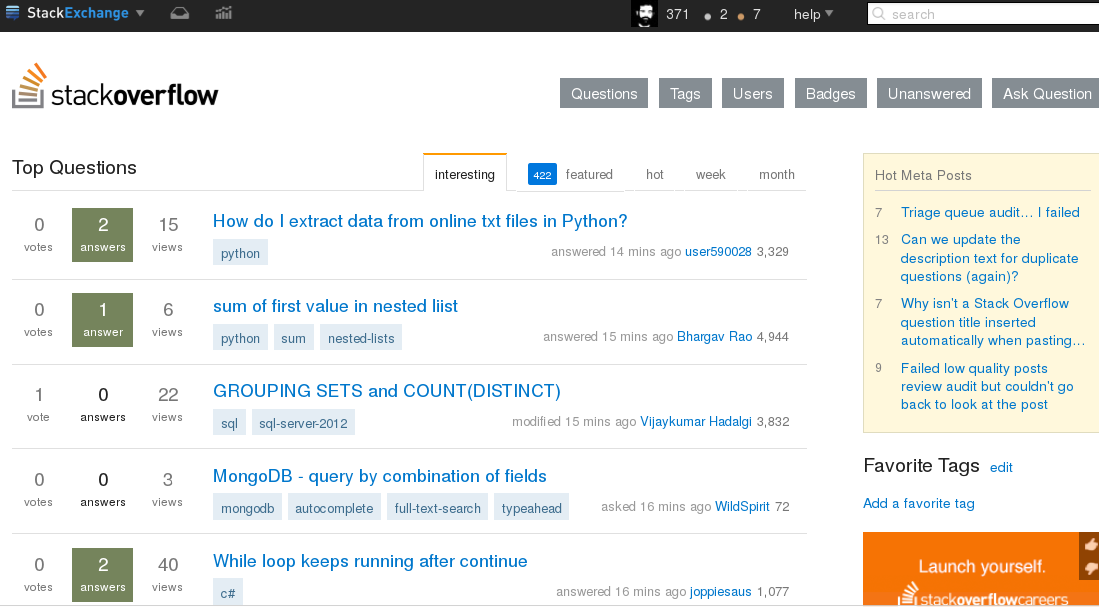
\includegraphics[height=7cm]{figs/sof}
\end{center}

\end{frame}


%%-----------------------------------------------------
\begin{frame}
\frametitle{Busca preguntas}

\begin{center}
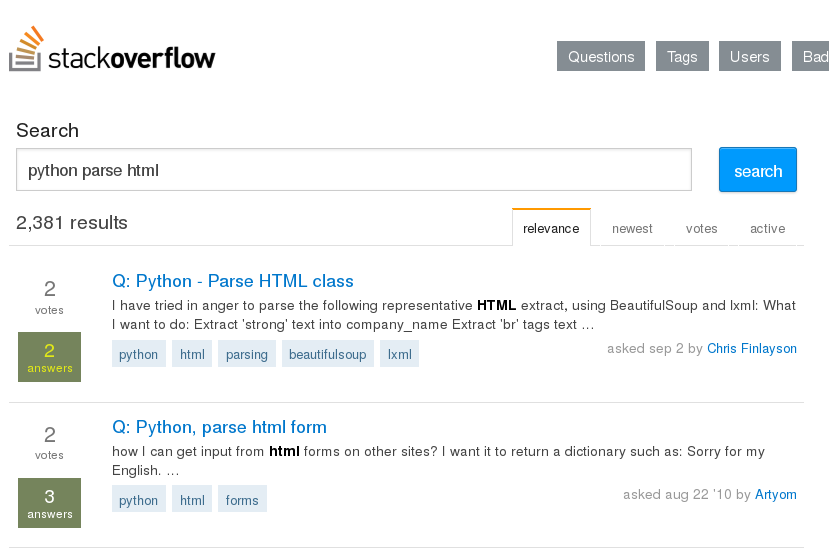
\includegraphics[height=7cm]{figs/sof-questions}
\end{center}

\end{frame}


%%-----------------------------------------------------
\begin{frame}
\frametitle{Encuentra respuestas}

\begin{center}
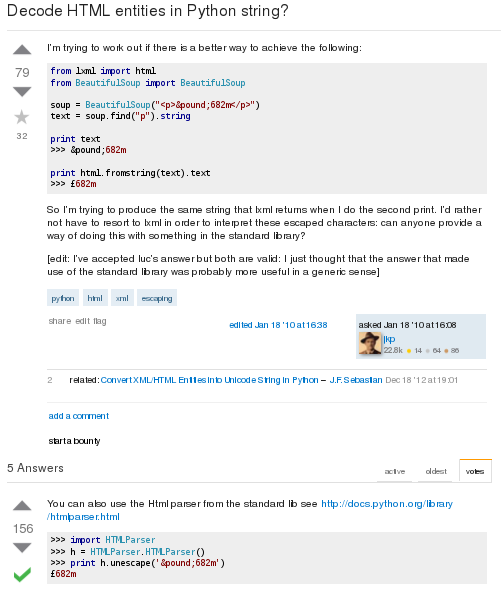
\includegraphics[height=7cm]{figs/sof-question}
\end{center}

\end{frame}

%%-----------------------------------------------------
\begin{frame}
\frametitle{Hazte una reputación}

\begin{center}
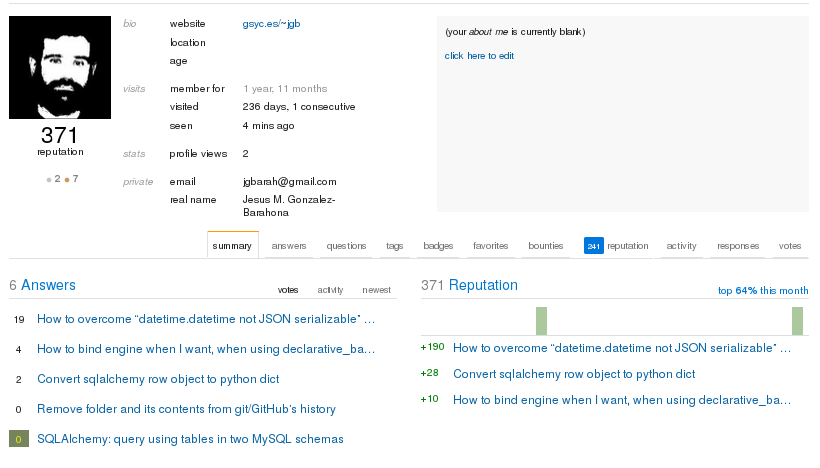
\includegraphics[height=7cm]{figs/sof-dashboard}
\end{center}

\end{frame}


 % jgb

% ST, jgb, 2022-02-03
%
%

%%-----------------------------------------------------
%%-----------------------------------------------------
\section{De rebajas}

%%-----------------------------------------------------
\begin{frame}
\frametitle{Markdown}

{\Large
\begin{itemize}
\item Primera version: 2004
\item Objetivo:
  \begin{quote}
  ``escribir usando un formato plano de texto, fácil de leer y fácil de escribir, que pueda ser convertido a HTML''
  \end{quote}
\item Uso creciente
\item Cada vez más herramientas
\item Cada vez más extensiones
\item README.md de GitHub
\end{itemize}
}

\begin{center}

\includegraphics[width=11cm]{figs/markdown-logo}
\end{center}

\end{frame}


%%-----------------------------------------------------
\begin{frame}[fragile]
\frametitle{Ejemplo (texto / HTML)}

\begin{columns}[T]
\begin{column}{.43\textwidth}

\begin{verbatim}
# Ejemplo

Esto es un pequeño ejemplo...

## Subtítulo

Ejemplos en los
[README.md de Git Hub]
(http://github.io "Git Hub")

Ejemplo de lista:
* Uno
* Dos
* Tres
\end{verbatim}

\end{column}%
\hfill%
\begin{column}{.53\textwidth}
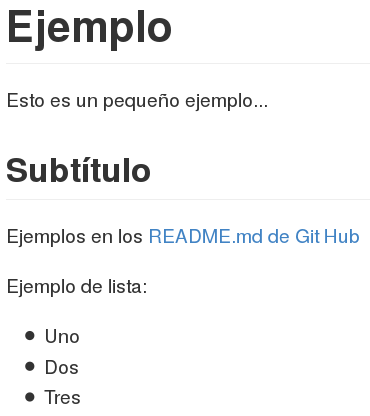
\includegraphics[width=6.5cm]{figs/markdown-ejemplo}
\end{column}%
\end{columns}

\end{frame}

%%-----------------------------------------------------
\begin{frame}
\frametitle{Marcado, herramientas}

Guías de marcado:
\begin{itemize}
\item Original \\
{\small \url{http://daringfireball.net/projects/markdown/syntax}} \\
\item GitHub \\
{\small \url{http://help.github.com/articles/github-flavored-markdown/}} \\
\item Pandoc \\
{\small \url{http://johnmacfarlane.net/pandoc/demo/example9/pandocs-markdown.html}} \\
\end{itemize}

Herramientas:
\begin{itemize}
\item Pandoc
\item Grip (Github Readme Instant Preview)
\item ...
\end{itemize}

\end{frame}

%%-----------------------------------------------------
\begin{frame}
\frametitle{Ejemplo: un libro con Markdown}

\begin{center}
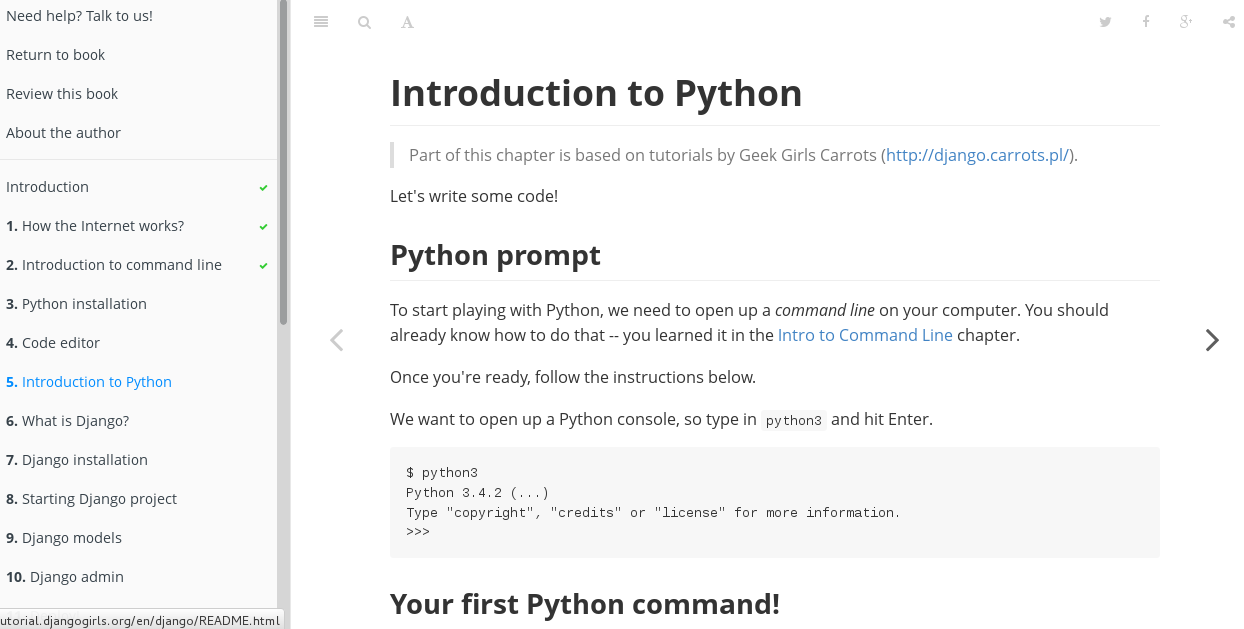
\includegraphics[width=11cm]{figs/markdown-book}
\end{center}

\begin{flushright}
\url{http://djangogirls.gitbooks.io/djangogirls-tutorial/} \\
\url{https://github.com/GitbookIO/gitbook} \\
\end{flushright}

\end{frame}
 % jgb

% SAT, SARO, 2022-02-01
\section{Trabajo top}

%-----------------------    ---------------------------------

\begin{frame}
\frametitle{¿Qué es un trabajo \emph{bueno}?}

\begin{itemize}
   \item Un trabajo que te permita ser creativo
   \item Un trabajo donde trabajes con últimas tecnologías
   \item Un trabajo donde puedas ascender sin dejar de ser ingeniero
   \item Un trabajo donde te paguen bien (y otros beneficios)
\end{itemize}

Hay muchas empresas donde buscan este tipo de perfil: Google, Apple, Facebook,
Microsoft, Yahoo!, Amazon...

\end{frame}

%-----------------------    ---------------------------------

\begin{frame}
\frametitle{Salarios en las compañías top}

\begin{center}
  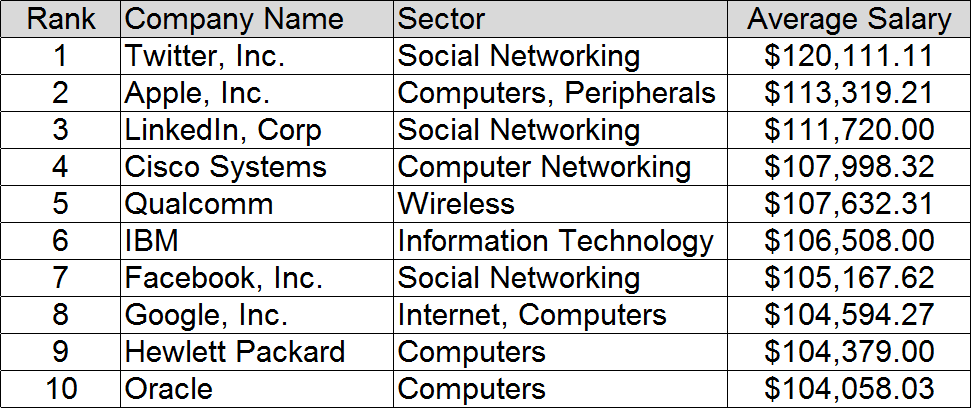
\includegraphics[width=10cm]{figs/toppaytech.png}
\end{center}


\begin{flushright}
{\tiny
http://img59.imageshack.us/img59/802/toppaytech.png
}
\end{flushright}

\end{frame}


%-----------------------    ---------------------------------

\begin{frame}
\frametitle{¿Qué te piden en estos trabajos?}

\begin{itemize}
   \item Estructuras de datos
   \item Algoritmia
   \item Experiencia en programación
   \item Redes de ordenadores
   \item Sistemas operativos
\end{itemize}

\end{frame}


%-----------------------    ---------------------------------

\begin{frame}
\frametitle{Más lecturas}

\begin{itemize}
   \item Hay varios libros sobre este tema, algunos en la biblioteca:
   \begin{itemize}
     \item Cracking the coding interview: 150 programming interview questions and solutions
     \item The Google Interview
     \item Elements of Programming Interviews: The Insiders' Guide
     \item Top 10 coding interview problems asked in Google with solutions: Algorithmic Approach
     \item Are You Smart Enough to Work at Google?: Fiendish Puzzles And Impossible Interview Questions From The World's Top Companies
     \item Get a Job WITHOUT an Interview - Google \& Beyond!: ``We don't mind to lose a good applicant, but definitely not hire a bad applicant.''
     \item The Google Resume: How to Prepare for a Career and Land a Job at Apple, Microsoft, Google, or any Top Tech Company
   \end{itemize}
\end{itemize}

\end{frame}



 % grex

% SAT, SARO, 2022-02-08
\section{MOOCs}

%-----------------------    ---------------------------------

\begin{frame}
\frametitle{¿Qué son los MOOCs?}

\begin{itemize}
   \item Cursos por Internet
   \item Hay algunos muy buenos, generalmente en inglés
   \item Generalmente gratis (algunos cobran por certificado, si lo terminas)
   \item Muchos de ellos ofrecidos por instituciones de renombre
   \item Basados generalmente en vídeos, lecturas y entrega de ejercicios
   \item Hay de todo: tecnológicos, de economía, de programación...
\end{itemize}

\end{frame}


%-----------------------    ---------------------------------

\begin{frame}
\frametitle{Sitios de MOOCs}

\begin{center}
  
\includegraphics[width=10cm]{figs/sitios.jpg}
\end{center}


\begin{flushright}
{\tiny
Source: http://www.vocal.ie/wp-content/uploads/2014/06/MOOCs-Daigram11.jpg
}
\end{flushright}

\end{frame}

%-----------------------    ---------------------------------

\begin{frame}
\frametitle{Plataformas recomendadas}

\begin{itemize}
   \item Coursera (existe la aplicación CourseraCast para ver los vídeos con el Chromecast en la TV)
   \item edX: del MIT
   \item Udacity: spin-off de Univ. Stanford
   \item MiríadaX (en español)
\end{itemize}

\end{frame}



 % grex

% SAT, SARO, 2022-02-15
\section{Educación de post-grado}

%-----------------------    ---------------------------------

\begin{frame}
\frametitle{Grado, Máster y Doctorado}


\begin{center}
  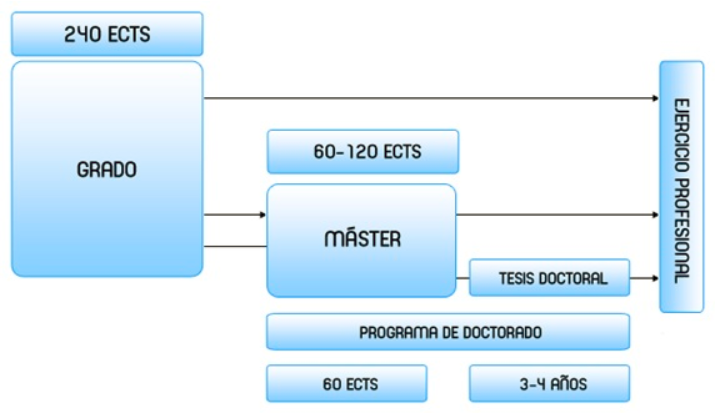
\includegraphics[width=10cm]{figs/post-grado.png}
\end{center}

\end{frame}

%-----------------------    ---------------------------------

\begin{frame}
\frametitle{¿En qué se diferencia un máster de un postgrado?}


\begin{center}
  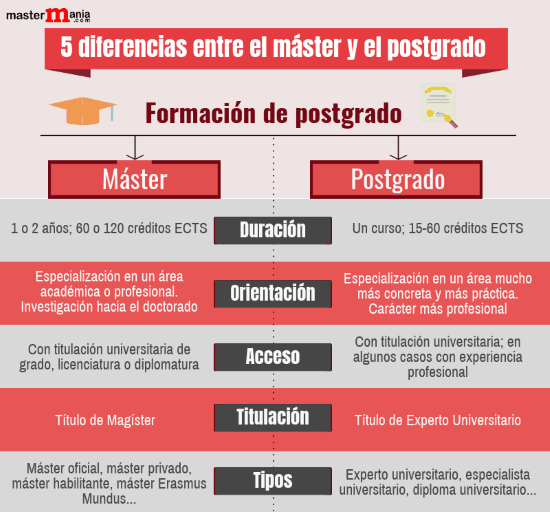
\includegraphics[width=7.5cm]{figs/diferencias_masterypostgrado.png}
\end{center}

\vspace{-0.8cm}
\begin{flushright}
{\tiny
Source: https://www.mastermania.com/noticias\_masters/que-diferencia-hay-entre-un-master-y-un-postgrado-org-5561.html
}
\end{flushright}

\end{frame}


%-----------------------    ---------------------------------

\begin{frame}
\frametitle{¿Qué es un máster oficial?}


\begin{center}
  
\includegraphics[width=8.5cm]{figs/master-oficial.jpg}
\end{center}

\vspace{-0.8cm}
\begin{flushright}
{\tiny
Source: https://www.educaweb.com/contenidos/educativos/masteres-posgrados/son-masteres-oficiales/
}
\end{flushright}

\end{frame}


%-----------------------    ---------------------------------

\begin{frame}
\frametitle{Tipos de máster}


\begin{center}
  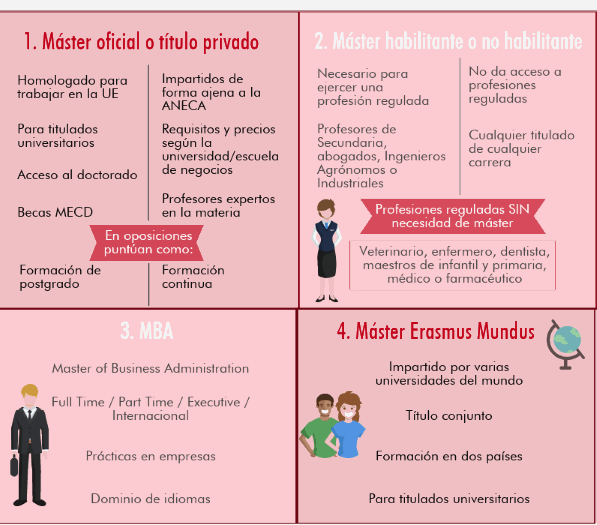
\includegraphics[width=8.3cm]{figs/tipos-master.png}
\end{center}

\vspace{-0.8cm}
\begin{flushright}
{\tiny
Source: https://www.mastermania.com/noticias\_masters/que-tipo-de-master-estudiar-presencial-distancia-u-online-org-5019.html
}
\end{flushright}

\end{frame}


%-----------------------    ---------------------------------

\begin{frame}
\frametitle{Tasa de empleo}


\begin{center}
  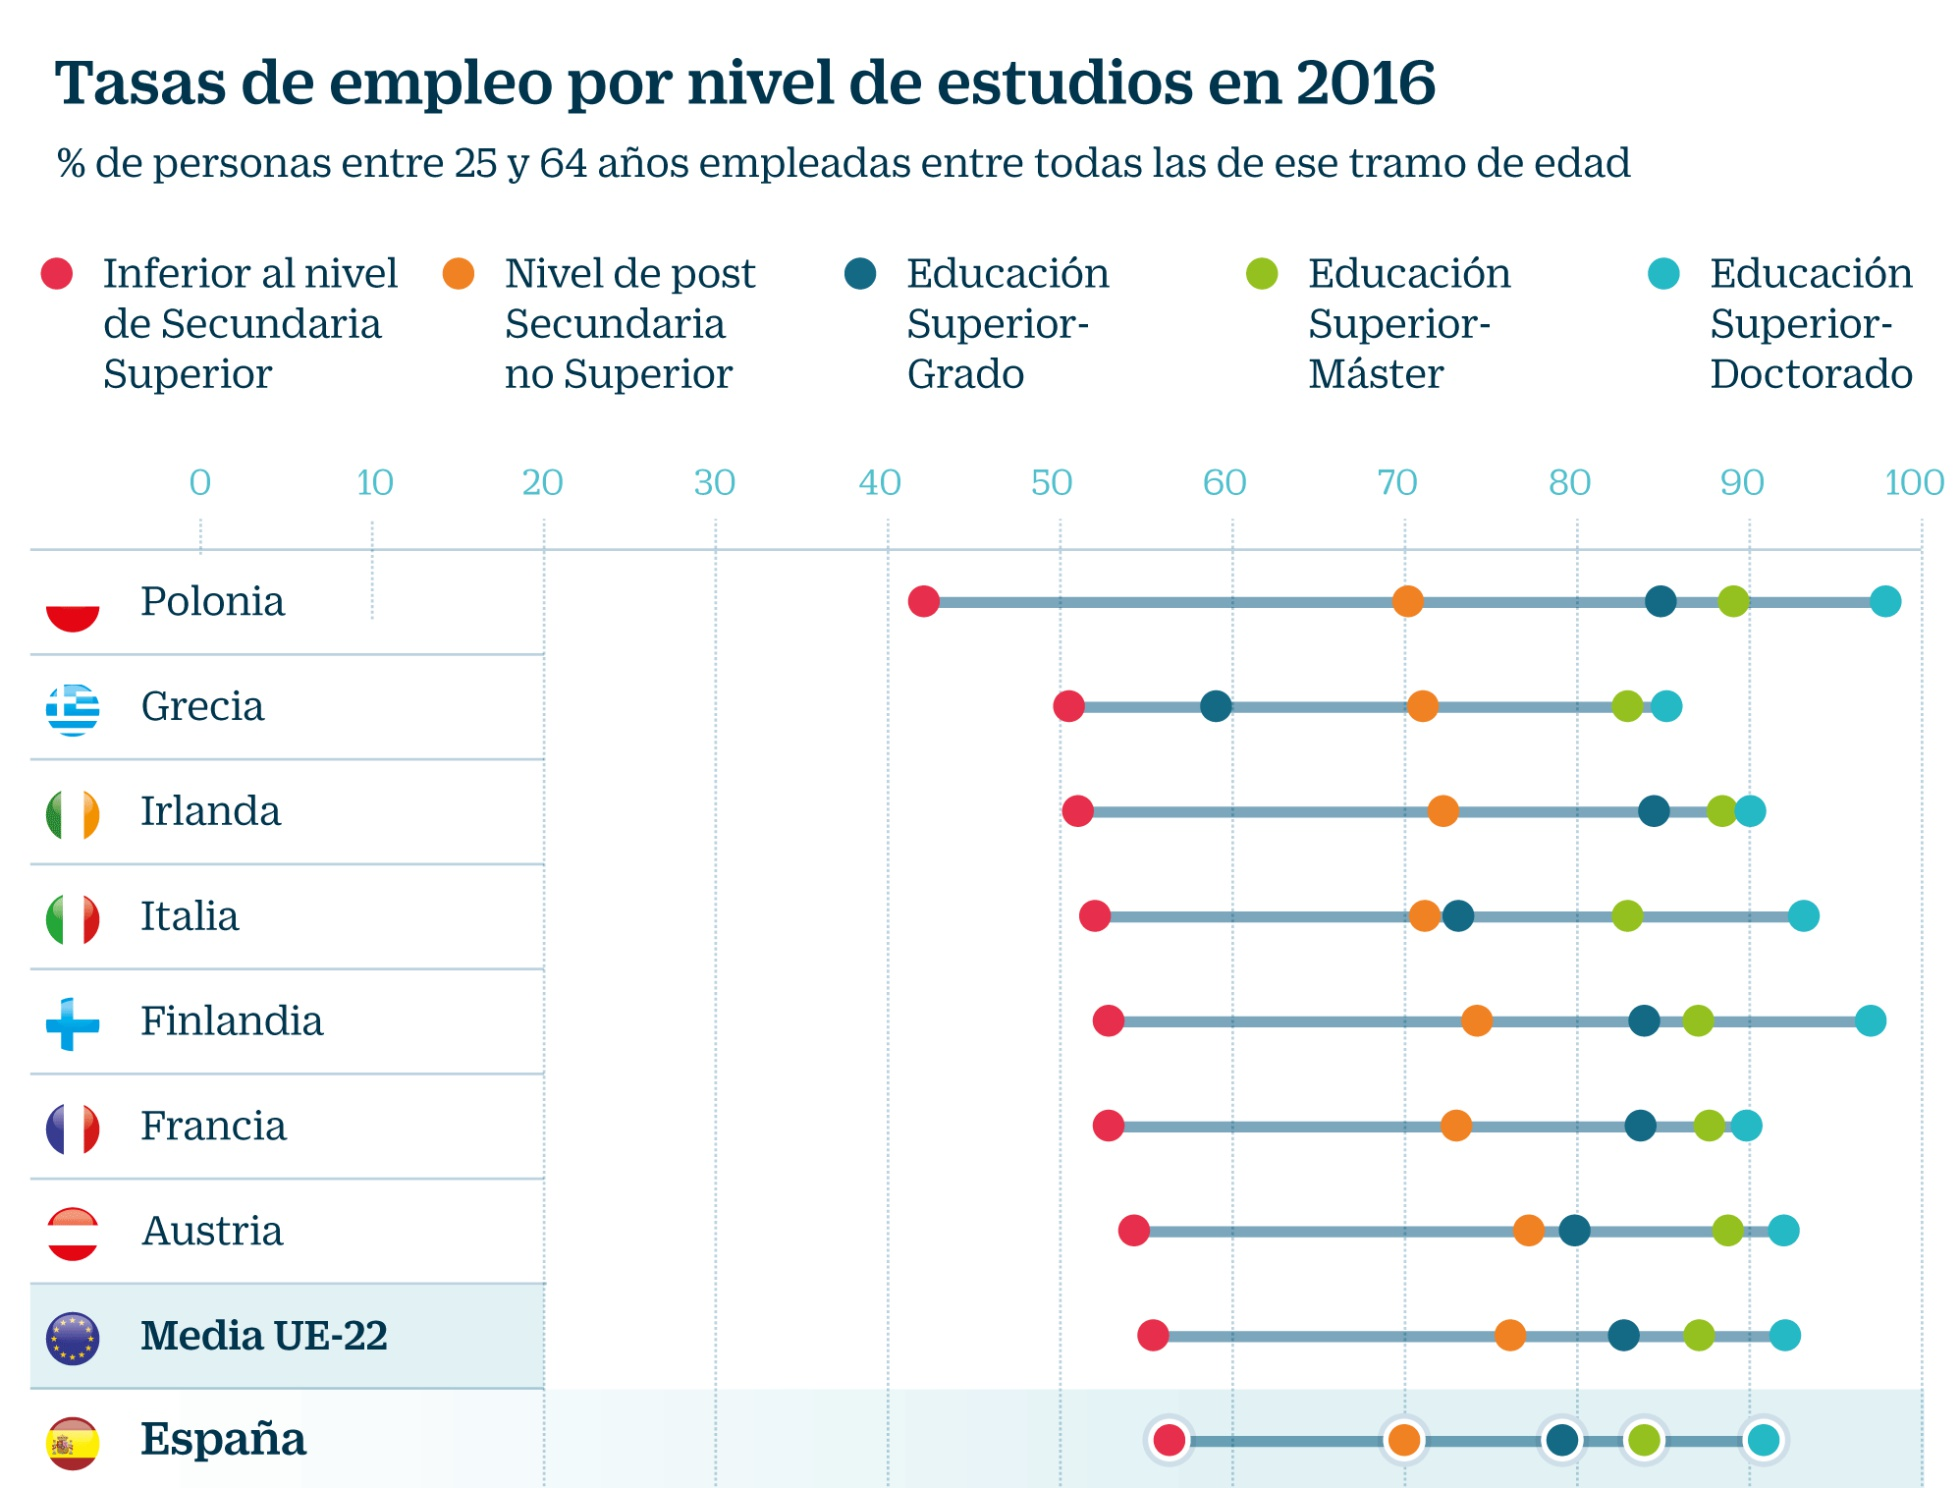
\includegraphics[width=9.8cm]{figs/tasa-empleo.jpg}
\end{center}

\vspace{-0.4cm}
\begin{flushright}
{\tiny
Source: https://cincodias.elpais.com/cincodias/2018/12/11/fortunas/1544552213\_155764.html
}
\end{flushright}

\end{frame}


%-----------------------    ---------------------------------

\begin{frame}
\frametitle{Salarios}


\begin{center}
  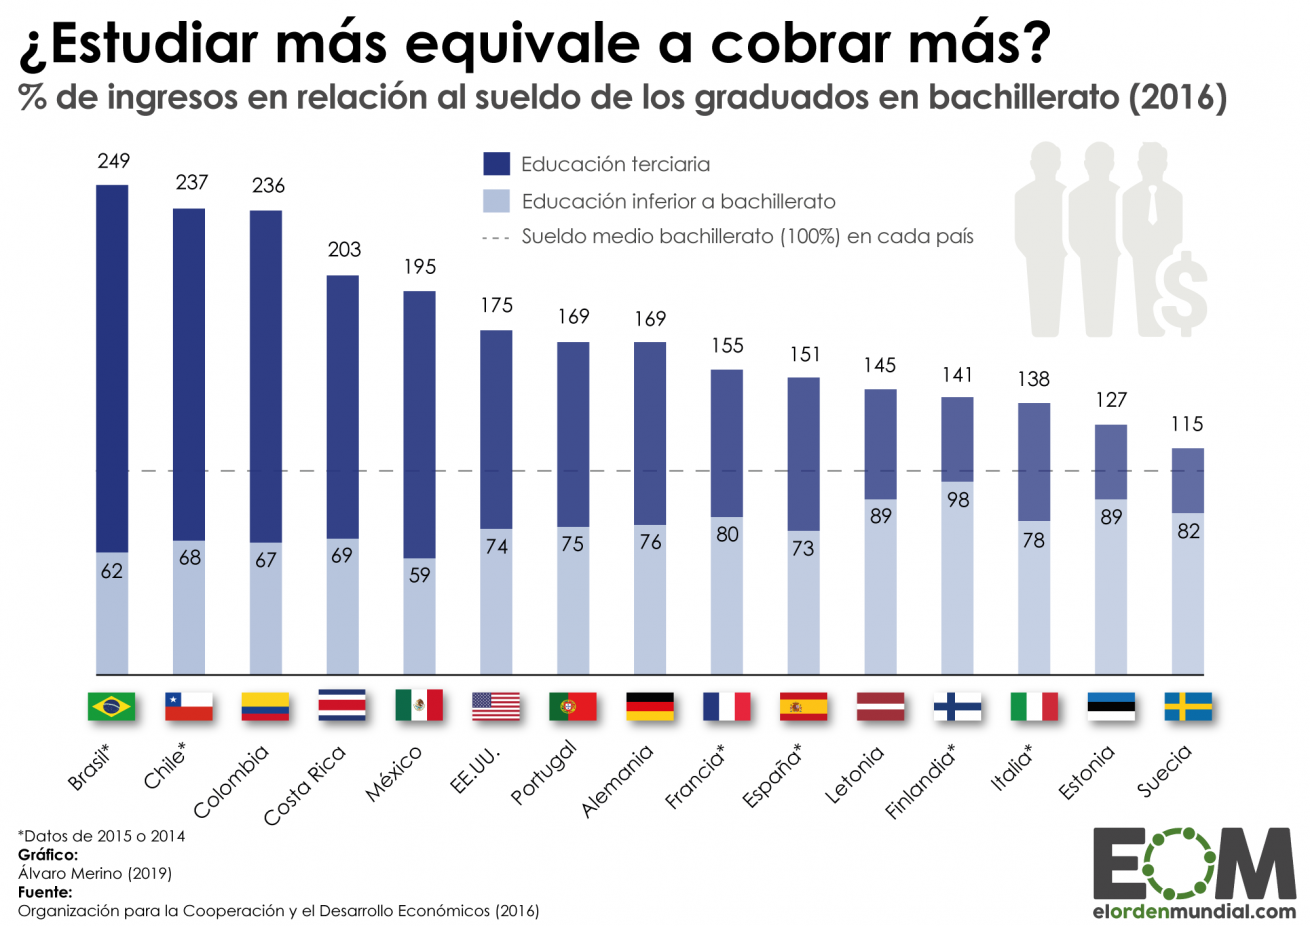
\includegraphics[width=9.8cm]{figs/salarios.png}
\end{center}

\vspace{-0.4cm}
\begin{flushright}
{\tiny
Source: https://elordenmundial.com/mapas-y-graficos/si-estudias-mas-cobraras-mas/
}
\end{flushright}

\end{frame}
 % grex

% ST, jgb, 2022-02-10
% SARO, jgb, 2022-02-10
%
%

%%-----------------------------------------------------
%%-----------------------------------------------------
\section{Lo importante es participar}

%%-----------------------------------------------------
\begin{frame}
\frametitle{Google Summer of Code}

\begin{columns}[T]
\begin{column}{.38\textwidth}

\includegraphics[width=6.5cm]{figs/gsoc-logo}

\begin{flushright}
{\small
\url{https://summerofcode.withgoogle.com/}
}
\end{flushright}

\end{column}%
\hfill%
\begin{column}{.60\textwidth}
{\Large
\begin{itemize}
\item Estudiantes post-secundaria
\item Mayores 18 años
\item Beca de 10 semanas meses (2.100 USD en 2021) 
\item Desarrollo para proyectos de software libre
\item Mentores en los proyectos
\item Dos selecciones: proyectos y becarios
\item Desde 2005
\end{itemize}
}
\end{column}%
\end{columns}

\end{frame}

%%-----------------------------------------------------
\begin{frame}
\frametitle{¿Quieres participar?}

{\Large

\begin{itemize}
\item Lee la documentación (empieza por las FAQ)
\item Mira ejemplos de otros años (hay muchos)
\item Elige tu proyecto, y tu idea de colaboración \\
  (comienza con las ideas propuestas)
\item Discute tu idea con el mentor potencial
\item Envía tu solicitud
\item Envía más detalles si te los piden
\end{itemize}

\begin{center}
¡Suerte!
\end{center}
}

\end{frame}

%%-----------------------------------------------------
\begin{frame}
\frametitle{¿Y qué gano si participo?}

{\Large

\begin{itemize}
\item Una buena tarjeta de visita \\
  Ser uno de los algo más de 1.000 GSOC anuales
\item La beca que te paga Google
\item Trabajar con proyectos reales en código real
\item Quizás, que incorporen tu código al proyecto
\item Conocer a tu mentor, y a otros desarrolladores
\end{itemize}

\begin{center}
Trabajar mucho, pasártelo bien
\end{center}
}

\end{frame}

%%-----------------------------------------------------
\begin{frame}
\frametitle{Outreachy}

{\Large

\begin{itemize}
\item Trabajo tuturizado en proyectos de software libre
\item Selección orientada a incrementar la diversidad
\item Funcionamiento similar a GSoC
\item Tres meses, 6.000 USD (2021)
\item Dos convocatorias al año
\end{itemize}

\vspace{1cm}

\begin{flushright}
  \url{https://www.outreachy.org/}
\end{flushright}
}

\end{frame}

 % jgb


% ST, jgb, 2022-02-17
% SARO, jgb, 2022-02-17
%
%

%%-----------------------------------------------------
%%-----------------------------------------------------
\section{La maravillosa Wayback Machine}

%%-----------------------------------------------------
\begin{frame}
\frametitle{¿Cómo era la web de la URJC?}


\includegraphics[height=6cm]{figs/web-urjc-2014}

{\Large
\begin{flushright}
2014
\end{flushright}
}
\end{frame}

%%-----------------------------------------------------
\begin{frame}
\frametitle{¿Cómo era la web de la URJC?}


\includegraphics[height=6cm]{figs/web-urjc-2011}

{\Large
\begin{flushright}
2011
\end{flushright}
}
\end{frame}

%%-----------------------------------------------------
\begin{frame}
\frametitle{¿Cómo era la web de la URJC?}

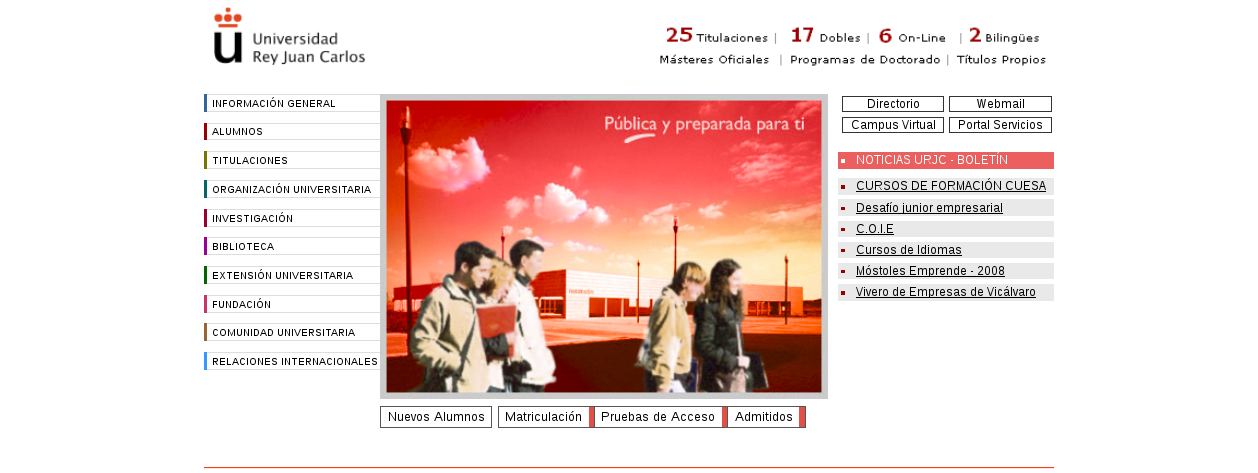
\includegraphics[height=6cm]{figs/web-urjc-2008}

{\Large
\begin{flushright}
2008
\end{flushright}
}
\end{frame}

%%-----------------------------------------------------
\begin{frame}
\frametitle{¿Cómo era la web de la URJC?}

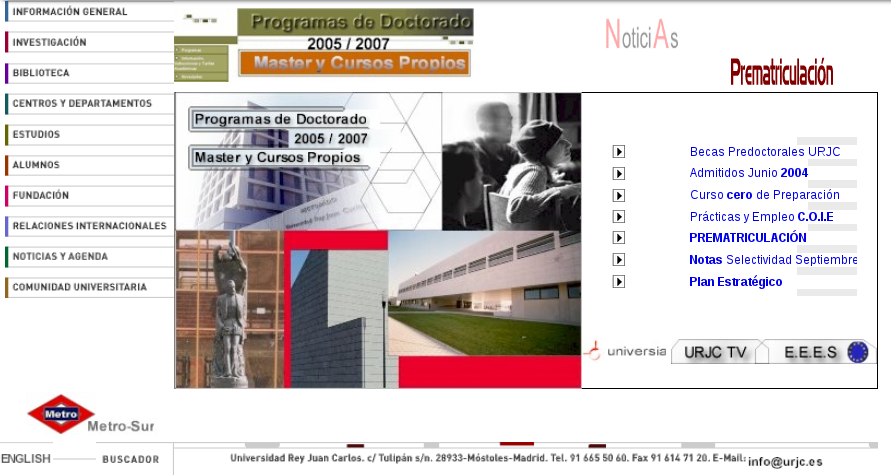
\includegraphics[height=6cm]{figs/web-urjc-2004}

{\Large
\begin{flushright}
2004
\end{flushright}
}
\end{frame}

%%-----------------------------------------------------
\begin{frame}
\frametitle{Bienvenidos a la maravillosa Wayback Machine}

{\Large
\begin{itemize}
\item Copias sitios web en distintos momentos del pasado
\item Parte del Internet Archive
\item Proporiciona una interfaz web...
\item ...y una API
\end{itemize}

\begin{flushright}
\url{https://archive.org/web/} \\
\url{https://archive.org/help/wayback_api.php} \\
\end{flushright}
}


\end{frame}


 % jgb

% ST, jgb, 2022-02-24
% SARO, jgb, 2022-02-24
%
%

%%-----------------------------------------------------
%%-----------------------------------------------------
\section{Mapas, mapas, mapas}

%%-----------------------------------------------------
\begin{frame}
\frametitle{OpenStreetMap}

\begin{center}
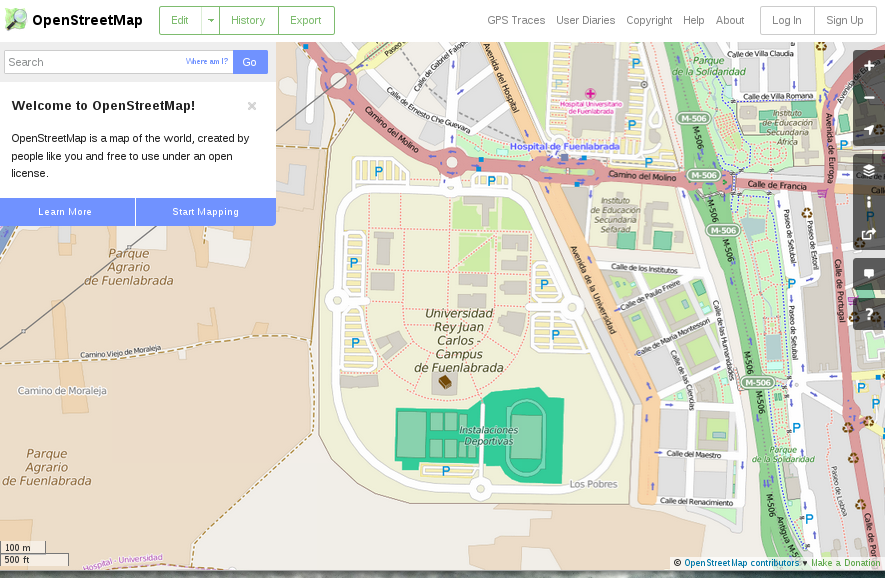
\includegraphics[height=7cm]{figs/openstreetmap}
\end{center}

\begin{flushright}
  \url{http://www.openstreetmap.org/}
\end{flushright}
\end{frame}

%%-----------------------------------------------------
\begin{frame}
\frametitle{OpenStreetMap (editando con iD)}

\begin{center}
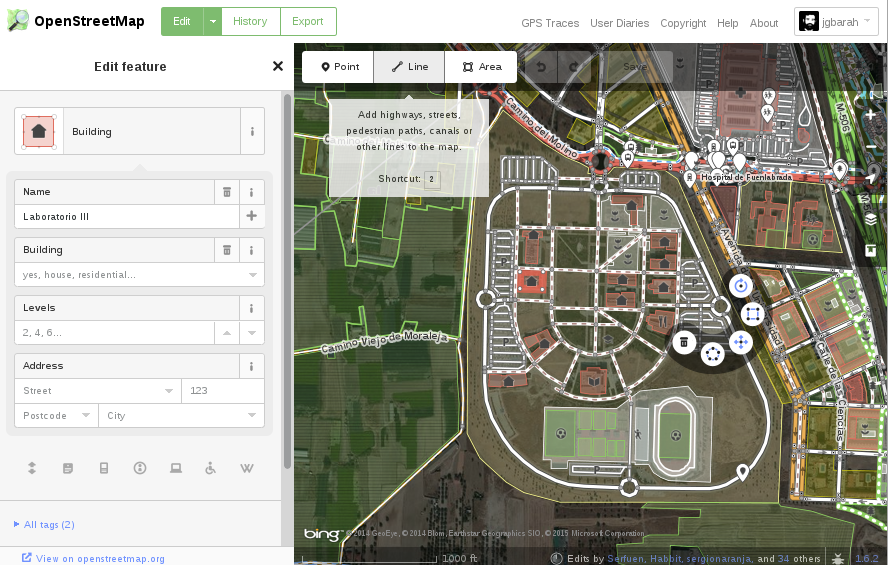
\includegraphics[height=7cm]{figs/openstreetmap-id}
\end{center}

\end{frame}


%%-----------------------------------------------------
\begin{frame}
\frametitle{Algunas curiosidades...}

\begin{itemize}
\item Servicios basdados en OpenStreetMap \\
  \url{http://wiki.openstreetmap.org/wiki/List_of_OSM-based_services} \\
\item Software que usa OpenStreetMap \\
  \url{http://wiki.openstreetmap.org/wiki/Software#Mobile_Devices} \\
\item Ejemplo de app Android: NavFree \\
  (permite off-line maps) \\
\item Cómo editar OpenStreetMap \\
  \url{https://www.youtube.com/watch?v=N_00vAPjSkw} \\
\item 10 años de OpenStreetMap (video) \\
  \url{https://www.youtube.com/watch?v=7sC83j6vzjo} \\
\end{itemize}

\end{frame}

 % jgb
\section{Licencias}

%-----------------------    ---------------------------------

\begin{frame}
\frametitle{¿Qué es la Propiedad Intelectual? ¿Y las licencias?}

\begin{itemize}
   \item La PI es la que regula qué se puede hacer con obras de carácter intelectual
   \item Se divide en dos partes
   \begin{itemize}
      \item Derechos morales (autoría, etc.). La mayoría irrenunciables y eternos
      \item Derechos de explotación (difusión, representación, copia...). Limitados en el tiempo.
   \end{itemize}
   \item Por defecto, el autor no te cede ningún derecho
   \item ... en la licencia vienen las condiciones de uso
\end{itemize}

\end{frame}


%-----------------------    ---------------------------------

\begin{frame}
\frametitle{Software libre}

\begin{enumerate}
  \setcounter{enumi}{-1}
   \item Permite su uso, con cualquier propósito
   \item Permite su estudio y su modificación
   \item Permite distribuir copias
   \item Permite mejorar y hacer públicas las mejoras.
\end{enumerate}

\begin{itemize}
  \item Hay muchas licencias de software libre: las más conocidas son la GNU GPL, la de Apache o las BSDs
  \item Hay licencias para otros contenidos (música, escritos...) como las Creative Commons
  \item El software libre no tiene por qué ser gratis.
  \item En GitHub, al iniciar un proyecto te pregunta por la licencia
\end{itemize}

\end{frame}

%-----------------------    ---------------------------------

\begin{frame}
\frametitle{Richard Stallman}

\begin{center}
  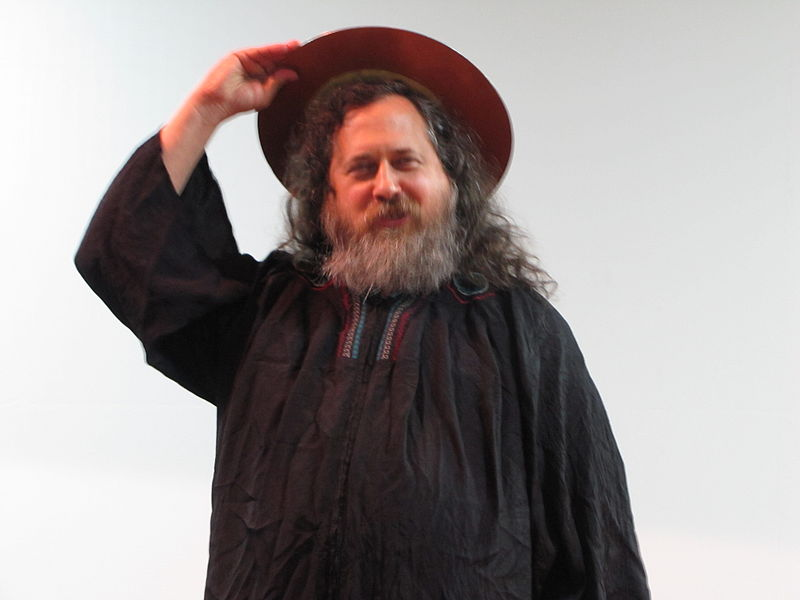
\includegraphics[width=10cm]{figs/stallman.jpg}
\end{center}


\begin{flushright}
{\tiny
Source: http://lunduke.com/wp-content/uploads/2012/03/RMS\_iGNUcius\_techfest\_iitb.jpeg
}
\end{flushright}

\end{frame}


 % grex

% ST, jgb, 2022-03-03
% SARO, jgb, 2022-03-03
%
%

%%-----------------------------------------------------
%%-----------------------------------------------------
\section{Ofusca, que algo queda}

%%-----------------------------------------------------
\begin{frame}[fragile]
\frametitle{No todo el código se escribe para que sea legible...}

Este programa escribe ``3.141'' calculando Pi a partir de su propia área.

{\tiny
\begin{verbatim}
#define _ -F<00||--F-OO--;
int F=00,OO=00;main(){F_OO();printf("%1.3f\n",4.*-F/OO/OO);}F_OO()
{
            _-_-_-_
       _-_-_-_-_-_-_-_-_
    _-_-_-_-_-_-_-_-_-_-_-_
  _-_-_-_-_-_-_-_-_-_-_-_-_-_
 _-_-_-_-_-_-_-_-_-_-_-_-_-_-_
 _-_-_-_-_-_-_-_-_-_-_-_-_-_-_
_-_-_-_-_-_-_-_-_-_-_-_-_-_-_-_
_-_-_-_-_-_-_-_-_-_-_-_-_-_-_-_
_-_-_-_-_-_-_-_-_-_-_-_-_-_-_-_
_-_-_-_-_-_-_-_-_-_-_-_-_-_-_-_
 _-_-_-_-_-_-_-_-_-_-_-_-_-_-_
 _-_-_-_-_-_-_-_-_-_-_-_-_-_-_
  _-_-_-_-_-_-_-_-_-_-_-_-_-_
    _-_-_-_-_-_-_-_-_-_-_-_
        _-_-_-_-_-_-_-_
            _-_-_-_
}
\end{verbatim}
}

\begin{flushright}
{\small
\url{http://www0.us.ioccc.org/years-spoiler.html#1988_westley}
}
\end{flushright}

\end{frame}

%%-----------------------------------------------------
\begin{frame}[fragile]
\frametitle{The International Obfuscated C Code Contest}

\begin{columns}[T]
\begin{column}{.63\textwidth}
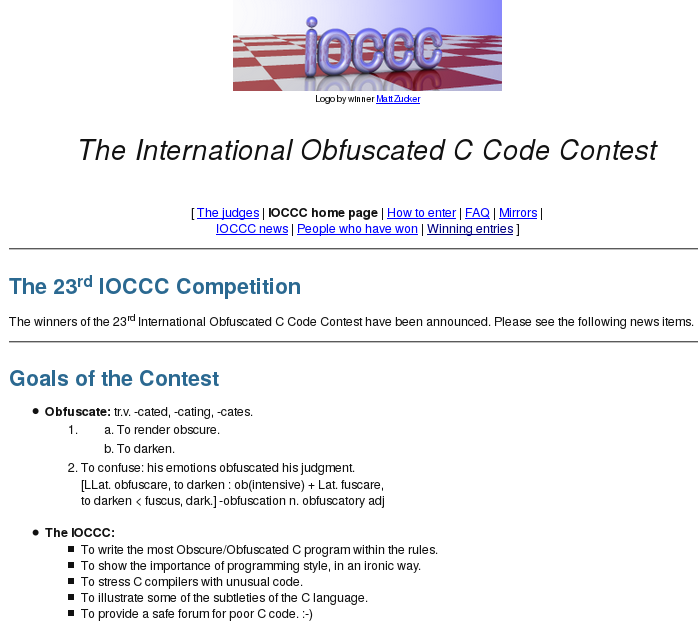
\includegraphics[width=8cm]{figs/obfuscated-ioccc}
\end{column}%
\hfill%
\begin{column}{.36\textwidth}
\begin{itemize}
\item Desde 1984
\item Celebrando la opacidad sintáctica \\
  (del lenguaje C)
\item \url{http://www.ioccc.org/}
\item Ganadores de cada concurso disponbiles
\end{itemize}
\end{column}%
\end{columns}


\begin{flushright}
{\footnotesize
\url{http://en.wikipedia.org/wiki/International_Obfuscated_C_Code_Contest}
}
\end{flushright}
\end{frame}

%%-----------------------------------------------------
\begin{frame}[fragile]
\frametitle{No sólo C, no sólo ofuscado (y también C y ofuscado)}

\begin{itemize}
\item Obfuscated Perl Contest \\
  Pero Perl es ruido de línea, ya sin ofuscar, ¿no?
\item Underhanded C Contest \\
  Código malicioso, pero que pasar un análisis riguroso
\item Weirdest obfuscated ``Hello World!'' \\
  StackExchange, ejemplos en varios lenguajes
\item IOCCC Flight Simulator \\
  ¡No me digas que no es maravilloso!
\end{itemize}

\begin{flushright}
{\small
\url{http://en.wikipedia.org/wiki/Obfuscated_Perl_Contest} \\
\url{http://www.underhanded-c.org/} \\
\url{http://codegolf.stackexchange.com/questions/22533/weirdest-obfuscated-hello-world} \\
\url{http://blog.aerojockey.com/post/iocccsim} \\
}
\end{flushright}
\end{frame}

%%-----------------------------------------------------
\begin{frame}
\frametitle{Mención aparte: Whitespace Programming Language}

\begin{center}
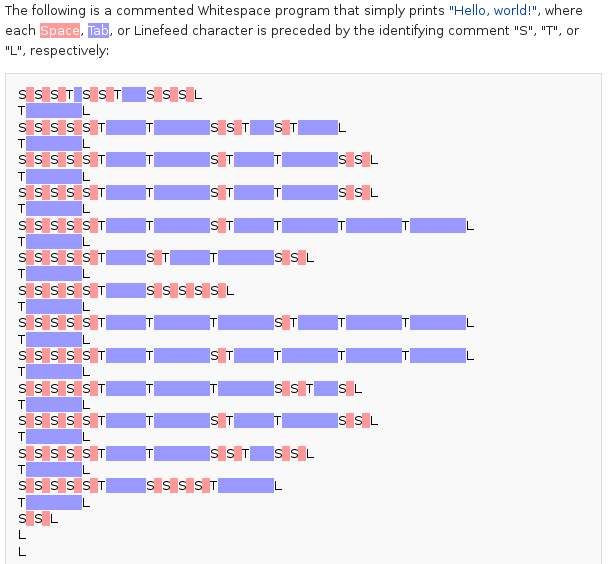
\includegraphics[width=7cm]{figs/obfuscated-whitespace}
\end{center}

\begin{flushright}
{\footnotesize
\url{http://compsoc.dur.ac.uk/whitespace/} \\
\url{http://en.wikipedia.org/wiki/Whitespace_\%28programming_language\%29}
}
\end{flushright}

\end{frame}

 % jgb

\section{Probando, probando...}

%-----------------------    ---------------------------------

\begin{frame}
\frametitle{¿Qué son los tests unitarios?}

\begin{itemize}
  \item Manera para determinar si el código funciona correctamente de manera automática
  \item Se separa el código de su respectiva prueba unitaria
  \item No prueba la falta de errores, pero bien hechos los minimiza
  \item Ideal para mejorar código que ya funciona y para trabajar en equipo
\end{itemize}

\end{frame}


%-----------------------    ---------------------------------

\begin{frame}
\frametitle{Frameworks}

\begin{itemize}
\item Hay \emph{frameworks} que te ayudan a hacerlos...
\item y hay \emph{frameworks} para todos los lenguajes de programación
\item El tradicional en Python3 es \texttt{unit.test}, aunque existen muchos otros
\item También se pueden hacer tests unitarios en Django
\end{itemize}

\end{frame}


%-----------------------    ---------------------------------

\begin{frame}[fragile]
\frametitle{Un ejemplo sencillo}

\begin{verbatim}
def contar_letra(cadena: str, letra: str) -> int:
    return cadena.count(letra)
\end{verbatim}

Función que dado un string \texttt{cadena}, devuelve el número de veces que
parece la letra \texttt{letra} en la cadena.

\end{frame}


%-----------------------    ---------------------------------

\begin{frame}[fragile]
\frametitle{Su test unitario}

\begin{verbatim}
import unittest
from contar import contar_letra

class Pruebas(unittest.TestCase):
    def test_contar_letra(self):
        self.assertEqual(contar_letra("pepe", "e"), 2)
        self.assertEqual(contar_letra("Madrid", "d"), 2)
        self.assertEqual(contar_letra("Un, dos", "o"), 1)        

if __name__ == '__main__':
    unittest.main()
\end{verbatim}

\end{frame}

%-----------------------    ---------------------------------

\begin{frame}[fragile]
\frametitle{Ejecución}

\begin{verbatim}
$ python3 test.py 
.
----------------------------------------------------------------------
Ran 1 test in 0.000s

OK
\end{verbatim}

\end{frame}

%-----------------------    ---------------------------------

\begin{frame}[fragile]
\frametitle{Su test unitario}

\begin{verbatim}
import unittest
from contar import contar_letra

class Pruebas(unittest.TestCase):
    def test_contar_letra(self):
        self.assertEqual(contar_letra("pepe", "e"), 2)
        self.assertEqual(contar_letra("Madrid", "d"), 2)
        self.assertEqual(contar_letra("Un, dos", "o"), 2)        

if __name__ == '__main__':
    unittest.main()
\end{verbatim}

\end{frame}


%-----------------------    ---------------------------------

\begin{frame}[fragile]
\frametitle{Ejecución}

\begin{verbatim}
$ python3 test.py 
F
======================================================================
FAIL: test_contar_letra (__main__.Pruebas)
----------------------------------------------------------------------
Traceback (most recent call last):
  File "test.py", line 8, in test_contar_letra
    self.assertEqual(contar.contar_letra("Un, dos", "o"), 2)
AssertionError: 1 != 2

----------------------------------------------------------------------
Ran 1 test in 0.000s

FAILED (failures=1)
\end{verbatim}

\end{frame}



%%% Local Variables:
%%% mode: latex
%%% TeX-master: "frikiminutos"
%%% End:
 % grex
%
%

%%-----------------------------------------------------
%%-----------------------------------------------------
\section{¿Qué datos tuyos tienen?}

%%-----------------------------------------------------
\begin{frame}
\frametitle{Un ejemplo: Facebook}

\begin{columns}[T]
\begin{column}{.65\textwidth}

\includegraphics[width=8cm]{figs/facebook-offsite}

\begin{flushright}
{\footnotesize
\url{https://www.facebook.com/off_facebook_activity}
}
\end{flushright}

\end{column}%
\hfill%
\begin{column}{.32\textwidth}
  Puedes consultar la información que Facebook tiene sobre ti...

  ...conseguida cuando estabas fuera de Facebook

  (gracias a los trackers de Facebook)
\end{column}%
\end{columns}

\end{frame}


%%-----------------------------------------------------
\begin{frame}
  \begin{center}
    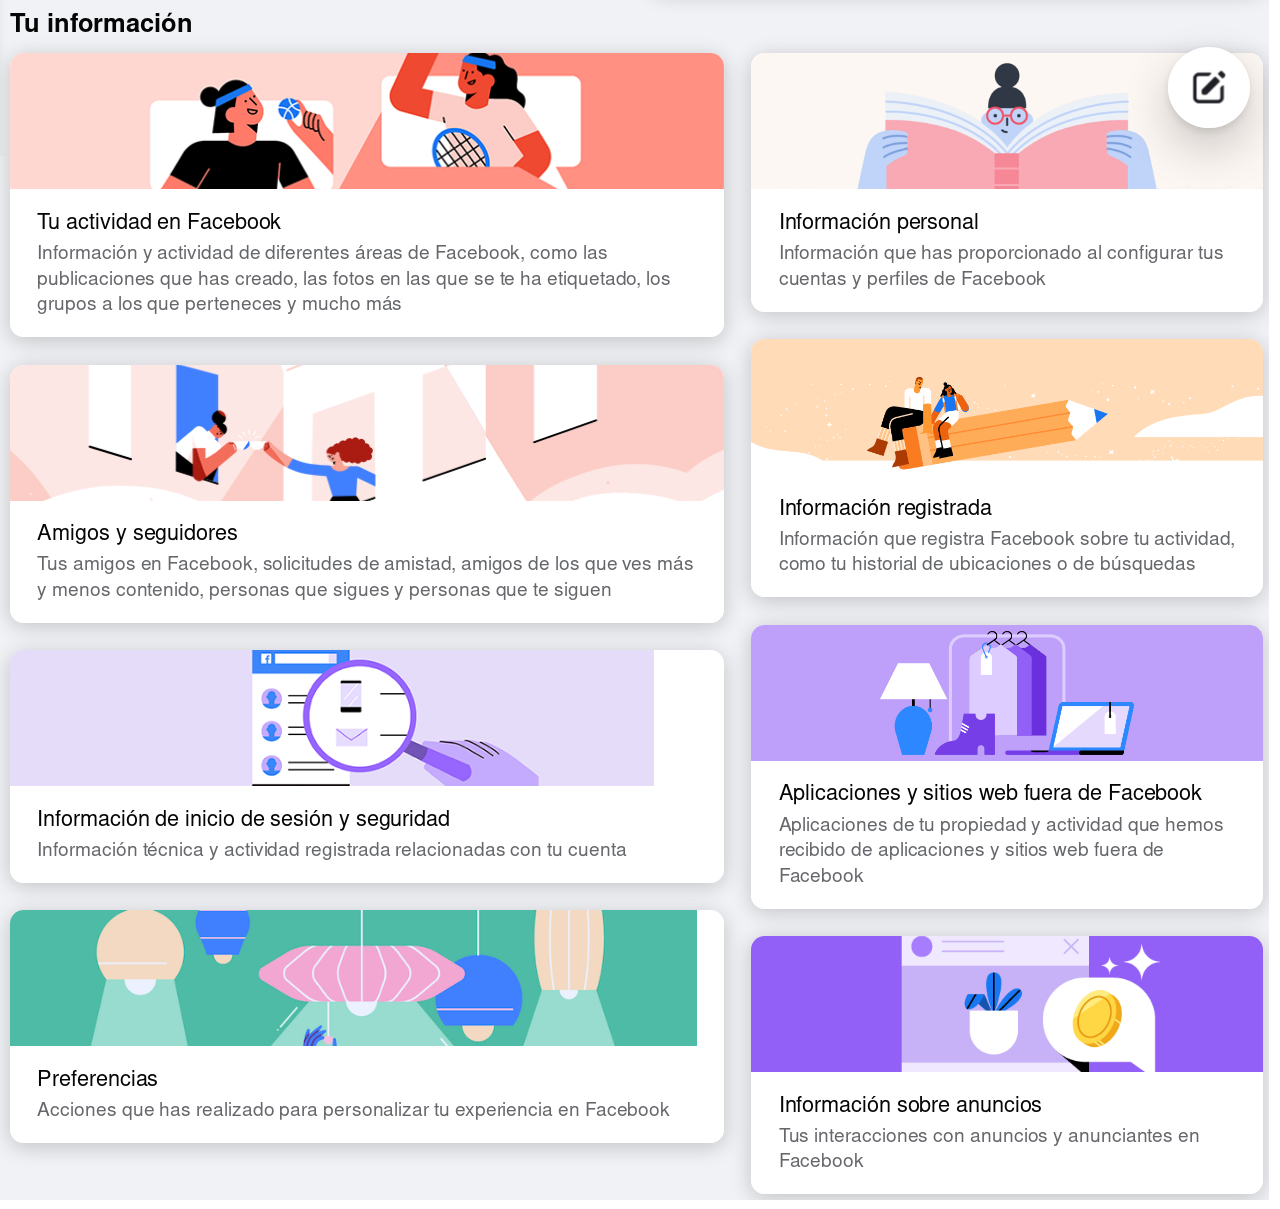
\includegraphics[width=8cm]{figs/facebook-offsite-2}
  \end{center}
\end{frame}


%%-----------------------------------------------------
\begin{frame}
  \frametitle{Más casos}

  {\Large
    
    Google:

    \begin{flushright}
      \url{https://myactivity.google.com}
    \end{flushright}

    Microsoft:
    
    \begin{flushright}
    \url{https://account.microsoft.com/privacy}
    \end{flushright}

    Amazon:
    
    \begin{flushright}
      \url{https://www.amazon.com/gp/help/customer/display.html?nodeId=GXPU3YPMBZQRWZK2}
    \end{flushright}
  }
\end{frame}
 %jgb
%
%

%%-----------------------------------------------------
%%-----------------------------------------------------
\section{Servidor web en Producción}

%%-----------------------------------------------------
\begin{frame}
\frametitle{Lo que enseñamos en clase}

\begin{columns}[T]
\begin{column}{.48\textwidth}
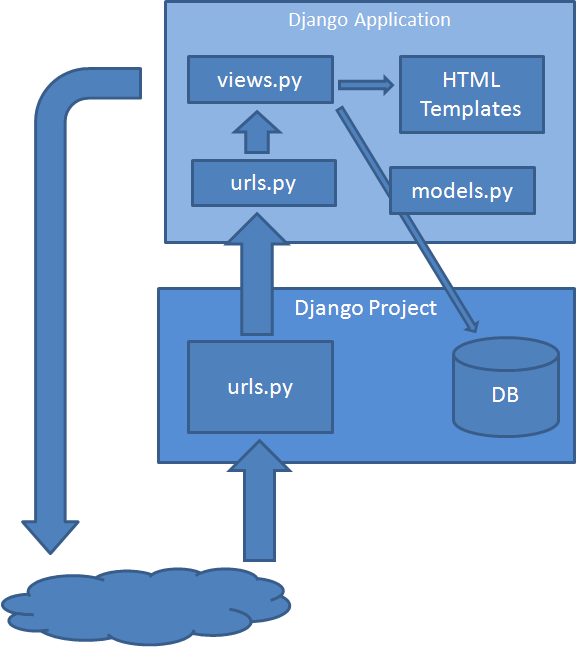
\includegraphics[width=6.5cm]{figs/django}

\begin{flushright}
  {\Large
    \url{http://django-project.com}
  }
\end{flushright}

\end{column}%
\hfill%
\begin{column}{.50\textwidth}
{\Large
\begin{itemize}
  \item Mono-hilo
  \item Mono-tarea
  \item Caché básico
  \item Base de datos limitada (sqlite)
  \item Pensado para páginas dinámicas
  \item Sin planificación
  \item No tiempo real
\end{itemize}
}
\end{column}%
\end{columns}

\end{frame}

%%-----------------------------------------------------
\begin{frame}
\frametitle{Un servidor web en producción}

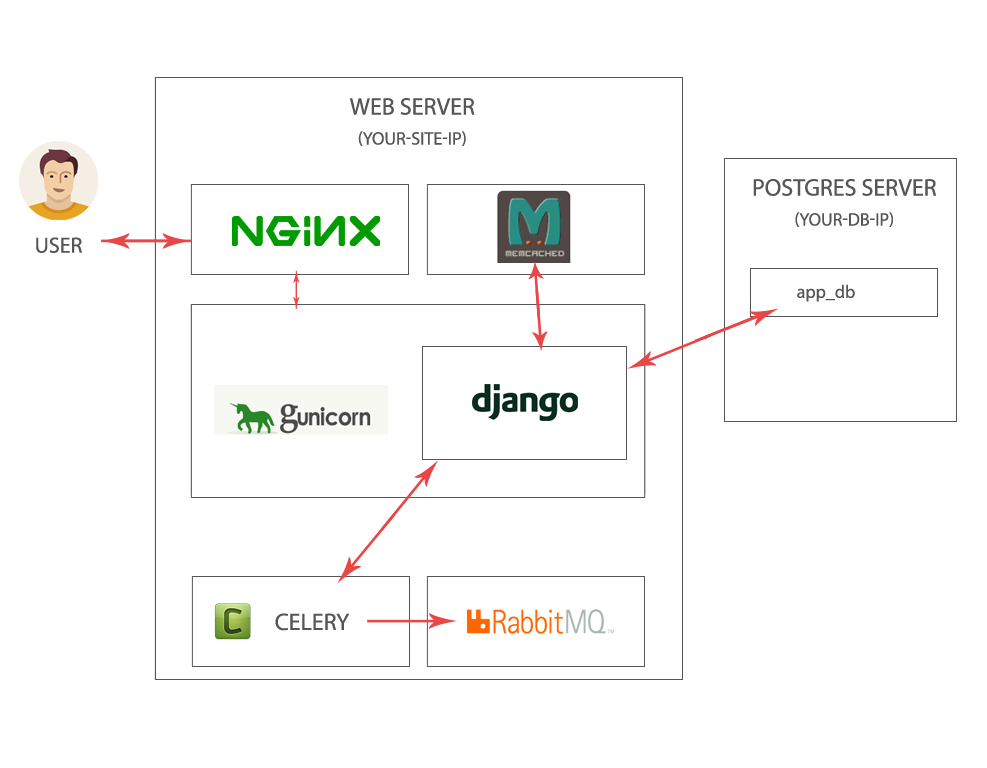
\includegraphics[width=11.5cm]{figs/django-y-mas} 

\end{frame}

%%-----------------------------------------------------
\begin{frame}
\frametitle{Tecnologías}

\begin{itemize}
  \item Django: Framework web
  \item Nginx: Servidor web con balanceo de carga (http://nginx.org/)
  \item Memcached: Caché (http://memcached.org/)
  \item gunicorn: Servidor HTTP (http://gunicorn.org/)
  \item Celery: Tiempo real y planificación de tareas (http://www.celeryproject.org/)
  \item RabbitMQ: Mensajería (https://www.rabbitmq.com/)
  \item PostgreSQL: Base de datos (http://www.postgresql.org/)
\end{itemize}

\end{frame}






 % grex
\section{Uso avanzado de la Shell}

%-----------------------    ---------------------------------

\begin{frame}
\frametitle{Acortadores de teclado}

\begin{itemize}
   \item \texttt{Tab}: autocompleta programas, ficheros y directorios
   \item \texttt{Ctrl+A}: va al principio de la línea
   \item \texttt{Ctrl+E}: va al final de la línea
   \item \texttt{Ctrl+R}: busca por lo intrducido en la historia
   \item \texttt{Ctrl+K}: borra desde el punto actual al final
   \item \texttt{Ctrl+U}: borra hasta el punto actual
   \item \texttt{Ctrl+L}: \emph{aclara} la pantalla (como el mandato \texttt{clear})
   \item \texttt{Alt+F}: se mueve a la siguiente palabra
   \item \texttt{Alt+B}: se mueve a la palabra anterior
\end{itemize}

(algunos se pueden configurar en el propio terminal)


\end{frame}


%-----------------------    ---------------------------------

\begin{frame}
\frametitle{Uso de pestañas}

\begin{center}
  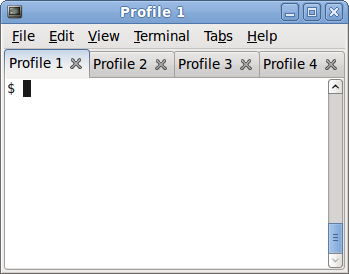
\includegraphics[width=4.5cm]{figs/tabs.png}
\end{center}


\begin{flushright}
{\tiny
http://unix.stackexchange.com/tags/gnome-terminal/info
}
\end{flushright}


\begin{itemize}
   \item Puedes poner nombre (título a cada pestaña)
   \item Nueva pestaña: \texttt{Ctrl+Alt+T} (yo lo suelo configurar como \texttt{Ctrl+T} para que sea igual que crear una nueva pestaña en el navegador)
   \item Pestaña siguiente/anterior: \texttt{Ctrl+PgUp} o \texttt{Ctrl+PgAbajo}
   \item \texttt{Alt+\emph{N}}: vas a la pestaña \emph{N}
\end{itemize}


\end{frame}


%-----------------------    ---------------------------------

\begin{frame}
\frametitle{Procesos}

\begin{itemize}
   \item \texttt{top}: Muestra los procesos según su \emph{consumo}
   \item \texttt{ps aux}: Lista todos los procesos del usuario
   \item \texttt{grep \emph{expr}}: Filtra por \emph{expr} 
   \item \texttt{ps aux | grep python}: Muestra la información de procesos que contengan \emph{python}
   \item \texttt{kill -9 \emph{pid}}: \emph{mata} el proceso con identificador \emph{pid}
\end{itemize}


\end{frame}


%-----------------------    ---------------------------------

\begin{frame}
\frametitle{Un pequeño chiste friqui para terminar}

\begin{center}
  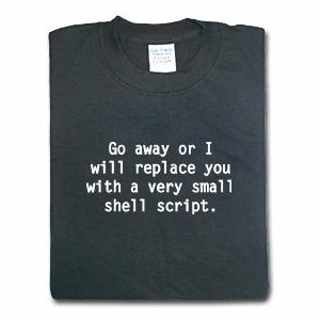
\includegraphics[width=7cm]{figs/shellscriptjoke.jpg}
\end{center}


\begin{flushright}
{\tiny
http://img819.imageshack.us/img819/4539/shellscriptjoke.jpg
}
\end{flushright}

\end{frame}



% ST, jgb, 2022-03-10
% SARO, jgb, 2022-03-10
\include{vm} % jgb



%%-----------------------------------------------------
%%-----------------------------------------------------
\section{IFTTT - If This Then That}


%-----------------------    ---------------------------------

\begin{frame}
\frametitle{¿Qué es IFTTT?}

\begin{itemize}
   \item Servicio web que permite enlazar condiciones sencillas (recetas) y que realizan cambios en otros servicios web
   \item Ejemplos:
   \begin{enumerate}
     \item Cuando llegue a casa/trabajo, activa la wifi
     \item Baja el volumen del teléfono cuando esté en clase
     \item Cada vez que envíe un tweet, guárdamelo en Google Docs
     \item Si me etiquetan en Facebook, guarda una copia en Instagram
     \item Enciende las luces cuando entre por el garaje
   \end{enumerate}
\end{itemize}

\end{frame}


%-----------------------    ---------------------------------

\begin{frame}
\frametitle{IFTTT}

\begin{center}
  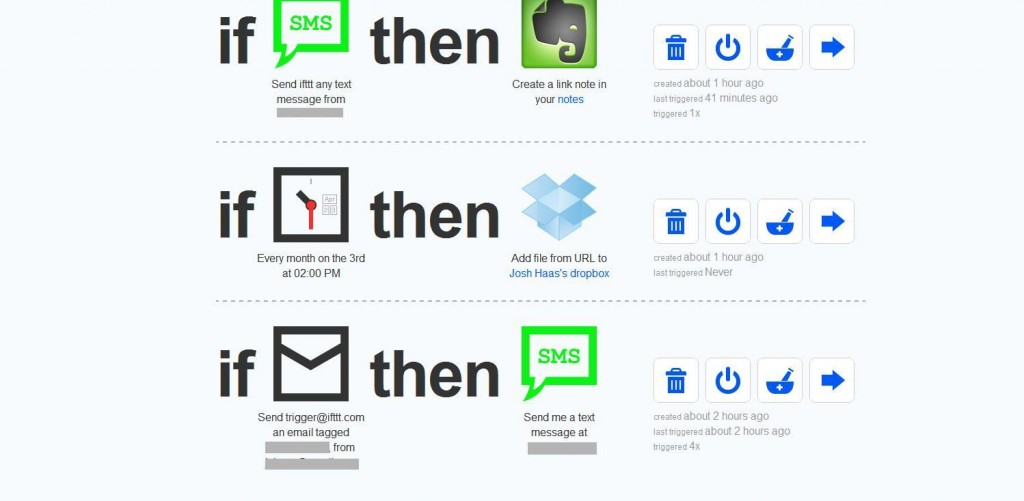
\includegraphics[width=13cm]{figs/if-recipes.jpg}
\end{center}


\begin{flushright}
{\tiny
Source: http://blog.joshhaas.com/2011/10/self-experimentation-using-ifttt-and-a-dash-of-python/
}
\end{flushright}

\end{frame}


%-----------------------    ---------------------------------

\begin{frame}
\frametitle{¿Por qué es interesante?}

\begin{itemize}
   \item La web no es sólo para humanos...
   \item Es un entorno distribuido multi-servicio
   \item Está adaptado al Internet de las cosas 
\end{itemize}

\end{frame}






% ST, jgb, 2022-03-17
% SARO, jgb, 2022-03-17
%
%

%%-----------------------------------------------------
%%-----------------------------------------------------
\usebackgroundtemplate{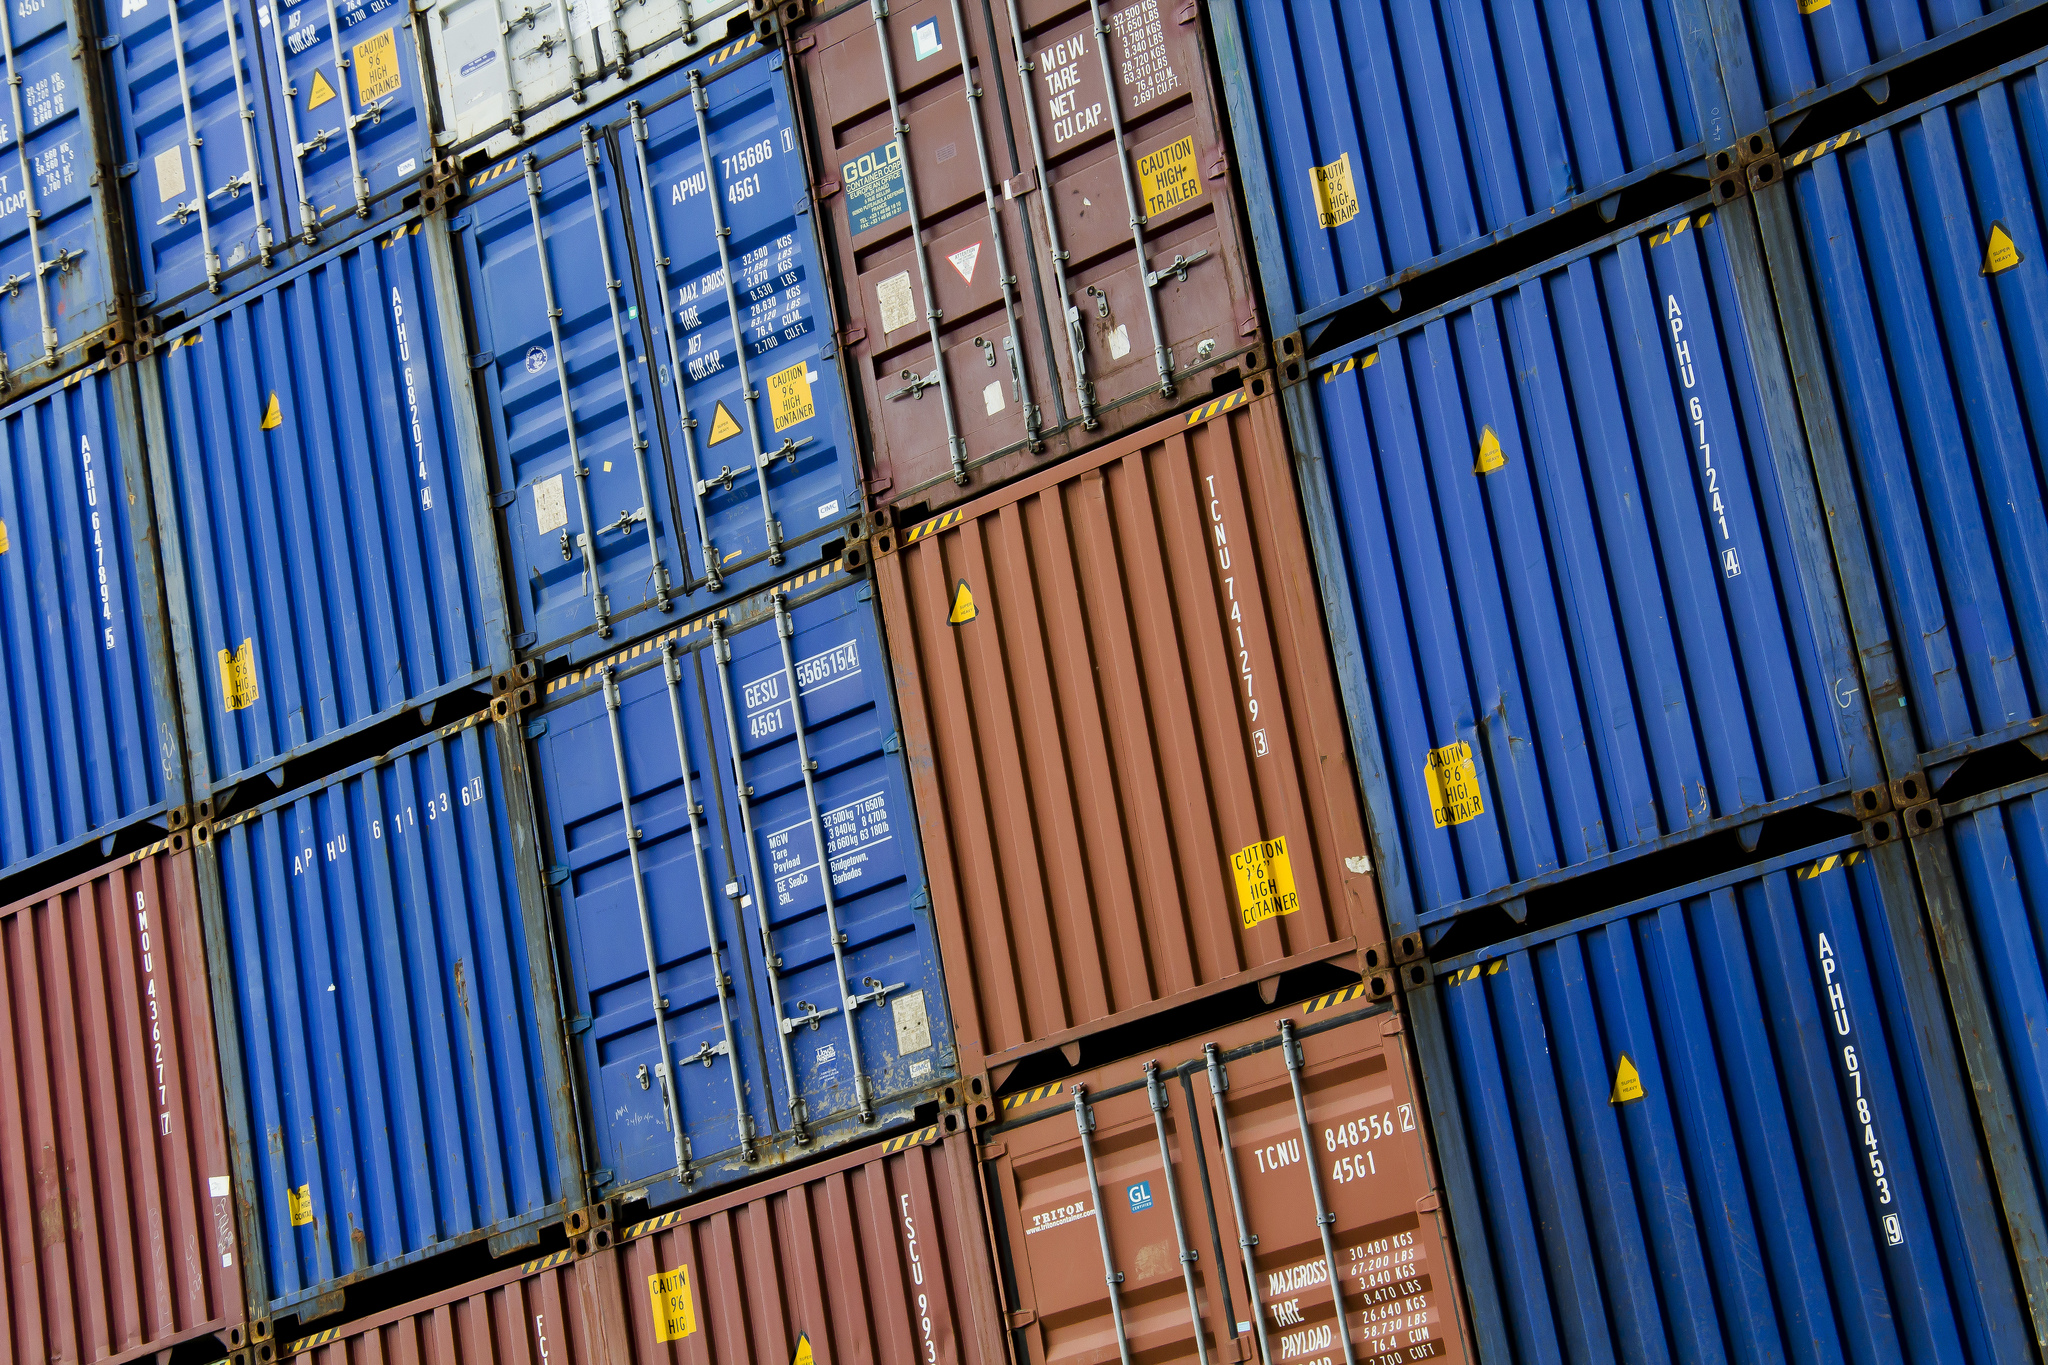
\includegraphics[width=\paperwidth,height=\paperheight]{figs/docker-containers.jpg}}
% Original figure: Flickr, Luke Price, ``Containers, Port of Rotterdam'', CC-by 2.0
% https://www.flickr.com/photos/lukeprice88/9703431992
{\bf
  \textcolor[rgb]{1,1,1}{
    \section{Contenedores por todas partes}
  }
}

\usebackgroundtemplate{}

%%-----------------------------------------------------
\begin{frame}
\frametitle{Contenedores software}

\begin{columns}[T]
\begin{column}{.48\textwidth}
{\Large
  \begin{itemize}
  \item Virtualización sobre sistema operativo
  \item Evolución de la idea de chroot
  \item Aislamiento \\
    (disco, memoria) \\
  \item Gestión de recursos
  \end{itemize}
}
\end{column}%
\hfill%
\begin{column}{.40\textwidth}
{\Large
  \begin{itemize}
  \item Más ligero que máquinas virtuales completas
  \item Mismo kernel \\
    que host \\
  \item Docker, LXC, LXD, \\
    FreeBSD Jail... \\
\end{itemize}
}
\end{column}%
\end{columns}

\end{frame}


%%-----------------------------------------------------
\begin{frame}
\frametitle{Docker (search trend)}

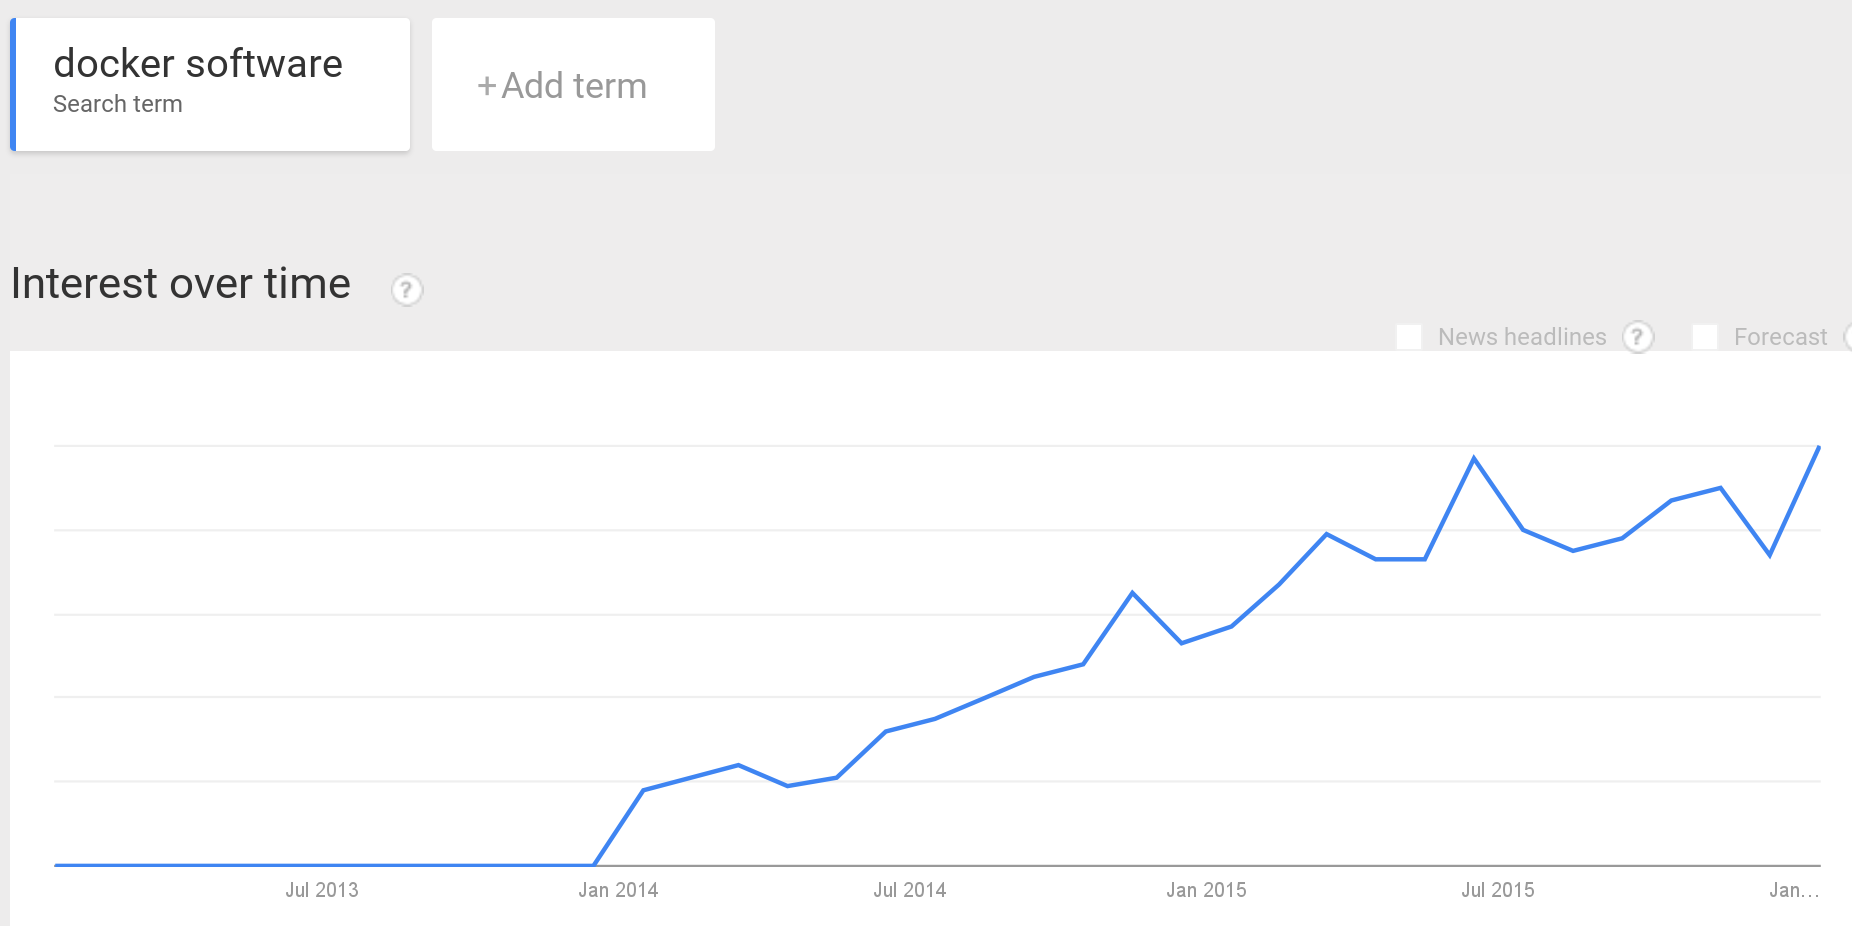
\includegraphics[width=12cm]{figs/docker-trend}


\end{frame}

%%-----------------------------------------------------
\begin{frame}
\frametitle{Docker}


\includegraphics[width=7cm]{figs/docker-logo}

\begin{columns}[T]
\begin{column}{.38\textwidth}

\begin{flushright}
{\Large
  \url{http://docker.com} 

  \vspace{1cm}

  \url{http://hub.docker.com/}
}
\end{flushright}

\end{column}%
\hfill%
\begin{column}{.60\textwidth}
{\Large
\begin{itemize}
\item Automatización del despliegue de aplicaciones en contenedores software
\item Montado sobre cgroups \\ (gestión de recursos), \\
  namespaces \\ (separación de recursos), \\
  sistema de ficheros con unión \\
\end{itemize}
}
\end{column}%
\end{columns}

\end{frame}

%%-----------------------------------------------------
\begin{frame}
\frametitle{Referencias y enlaces}

\begin{flushright}
  Luke Price, ``Containers, Port of Rotterdam'', CC-by 2.0 \\
  \url{https://www.flickr.com/photos/lukeprice88/9703431992} \\
\end{flushright}  

\end{frame}






 % jgb

% ST, jgb, 2022-03-31
% SARO, jgb, 2022-03-31
\include{openai} %jgb

\section{Pythonic}

\begin{frame}[fragile]
\frametitle{Esto es Python... ¿de verdad?}

\begin{verbatim}
countriesWithA = []
i = 0
while i < len(countryList):
   if "a" in countryList[i]:
      countriesWithA.append(countryList[i])
   i += 1
\end{verbatim}

\end{frame}


\begin{frame}[fragile]
\frametitle{Python... ¿mejor?}

\begin{verbatim}
countriesWithA = []
    
for i in range(len(countryList)):
   if "a" in countryList[i]:
      countriesWithA.append(countryList[i])
\end{verbatim}

\end{frame}


\begin{frame}[fragile]
\frametitle{Todavía más Pitónico}

\begin{verbatim}
countriesWithA = []

for country in countryList:
   if "a" in coutry:
      countriesWithA.append(country)
\end{verbatim}


\end{frame}


\begin{frame}[fragile]
\frametitle{Definitivamente Pitónico}

\begin{verbatim}
countriesWithA = [country for country in countryList 
                  if "a" in country]
\end{verbatim}

\end{frame}


\begin{frame}[fragile]
\frametitle{Pitónico Avanzado}

\begin{verbatim}
countriesWithA = (country for country in countryList
                  if "a" in country)
\end{verbatim}


\end{frame}


\begin{frame}
\frametitle{¿Qué es Pitónico?}

\begin{center}
{\Huge

\emph{Pitónico}

significa algo así como

\vspace{.3cm}

\emph{Python idiomático}.
}
\end{center}

\end{frame}

\begin{frame}
\frametitle{¿Qué es Python idiomático?}

{\Large

A medida que el lenguaje Python evoluciona y la comunidad crece, han surgido muchas ideas sobre cómo usar Python {\bf de  manera correcta}. 

}

\end{frame}

\begin{frame}
\frametitle{Pitónico es cultural}

{\Large

El lenguaje Python fomenta activamente una gran cantidad de modismos para realizar una serie de tareas {\bf (``una única forma de hacerlo'')}. 

}

\end{frame}

\begin{frame}
\frametitle{Python idioms}

Hay cientos de \emph{idioms} en Python

Aquí, algunas de las \emph{familias} de \emph{idioms}:

  \begin{columns}[T]
    \begin{column}{.5\textwidth}
     \begin{block}{}

\begin{itemize}
  \item \{List, Dictionary, Set\} comprehensions
  \item Magic methods
  \item Keyword arguments
  \item Properties
  \item Lambda functions
  \item Context managers
  \item Decorators
\end{itemize}

    \end{block}
    \end{column}
    \begin{column}{.5\textwidth}
    \begin{block}{}


\begin{itemize}
  \item Estructuras definidas en \texttt{collections}
  \item Static methods y classes
  \item Class methods
  \item Generators
  \item Uso de métodos específicos
  \item ...    
  \item ...
\end{itemize}

    \end{block}
    \end{column}
  \end{columns}

\end{frame}


\begin{frame}
\frametitle{Resumiendo...}

\begin{enumerate}
  \item Hay una cultura tras el lenguaje de Python
  \item El lenguaje de Python evoluciona siguiendo esta cultura
  \item Sabes algo de Python, pero el que sabes es poco pitónico
\end{enumerate}

\end{frame}


 % grex
%
%

%%-----------------------------------------------------
%%-----------------------------------------------------
\section{Texto para todos los gustos}

%%-----------------------------------------------------
\begin{frame}
\frametitle{Unicode}

\begin{columns}[T]
\begin{column}{.48\textwidth}

\includegraphics[width=5cm]{figs/unicode-logo}

\vspace{.5cm}

{\Large

\begin{flushright}
\url{http://unicode.org/}
\end{flushright}
}

\end{column}%
\hfill%
\begin{column}{.60\textwidth}
  {\Large
    Meta: texto en cualquier sistema de escritura
    
    \begin{itemize}
    \item codificación
    \item representación
    \end{itemize}

    \vspace{.2cm}
    
    \begin{itemize}
    \item 129 sistemas de escritura
    \item conjuntos de otros símbolos
    \item más de 120.000 caracteres
    \end{itemize}
  }
\end{column}%
\end{columns}

\end{frame}

%%-----------------------------------------------------
\begin{frame}
\frametitle{Principios}

{\Large
\begin{itemize}
\item Se codifican los grafemas (definición abstracta)
\item No trata sobre la representación
\item Cada grafema, un número (31 bits) \\
  Ejemplo: U+00F1 (ñ) \\
\item U+0000 -- U+00FF: Latin-1
\end{itemize}

\vspace{.2cm}

Codificaciones:

\begin{itemize}
\item UTF-8: anchura variable, compatible con ASCII
\item UTF-16: anchura variable, mejor para ideogramas
\item UTF-32: anchura fija
\end{itemize}
}

\end{frame}

%%-----------------------------------------------------
\begin{frame}
\frametitle{Primeros caracteres}

\begin{center}
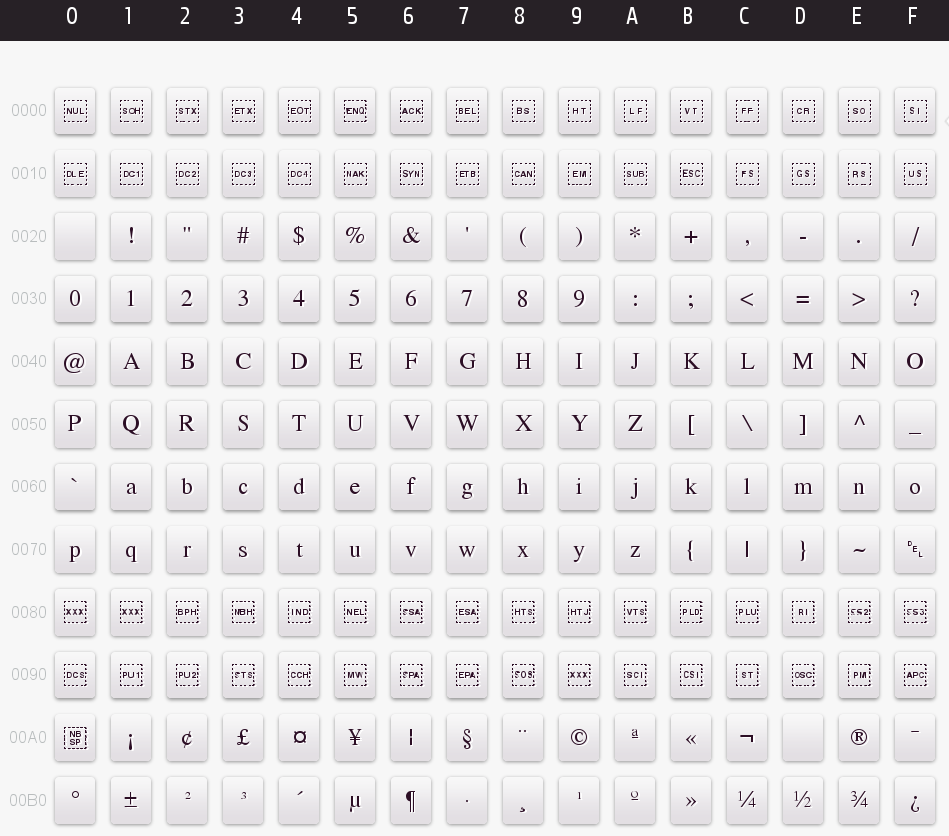
\includegraphics[width=9cm]{figs/unicode-0000}
\end{center}

\end{frame}

%%-----------------------------------------------------
\begin{frame}
\frametitle{Caracteres arábicos}

\begin{center}
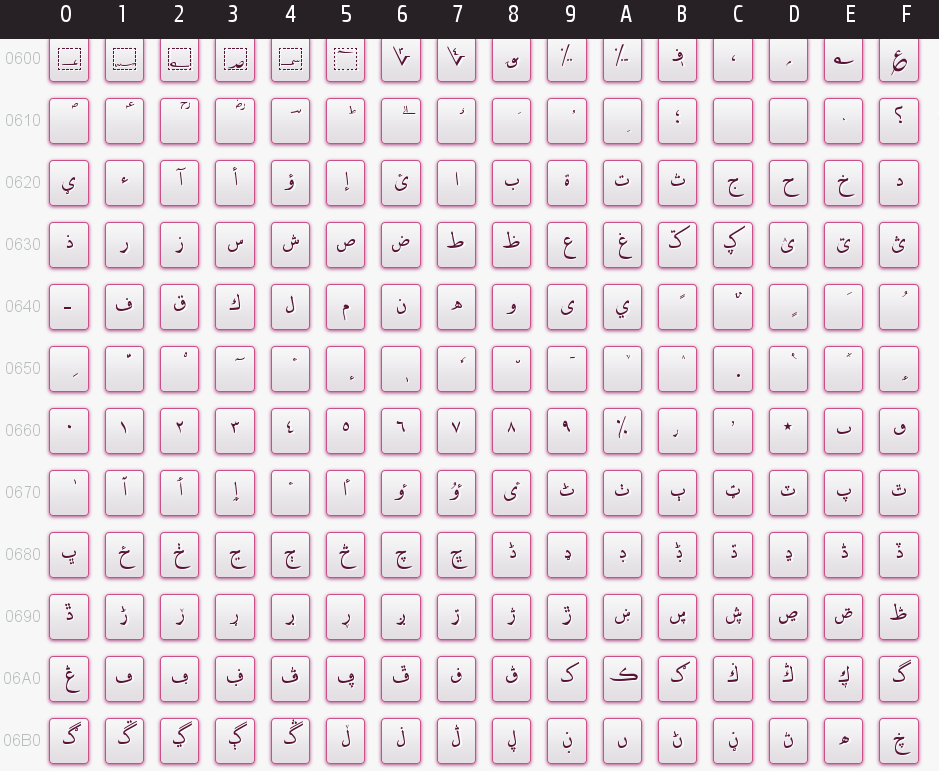
\includegraphics[width=9cm]{figs/unicode-0600}
\end{center}

\end{frame}

%%-----------------------------------------------------
\begin{frame}
\frametitle{Emojis}

\begin{center}
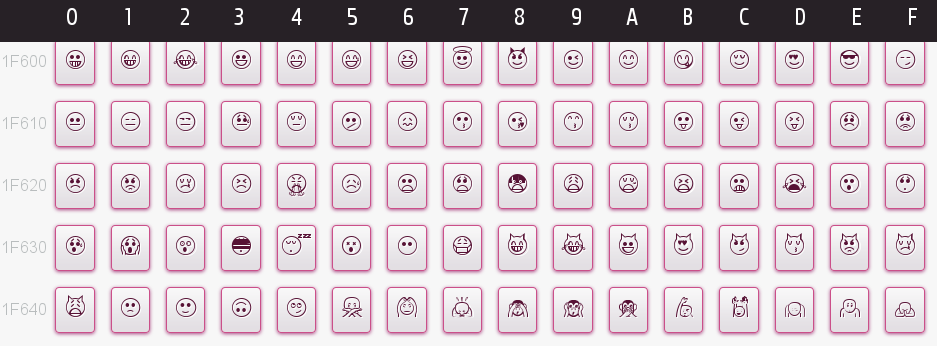
\includegraphics[width=9cm]{figs/unicode-emoji}
\end{center}

\begin{flushright}
  \url{http://unicode-table.com}
\end{flushright}
\end{frame}

 % jgb
\section{Accesibilidad en la web}

%-----------------------    ---------------------------------

\begin{frame}
\frametitle{¿Por qué accesibilidad?}

\begin{itemize}
   \item El porcentaje de ciudadanos en España con algún tipo de discapacidad se estima en el 9\% (INE 2002), aunque en USA se eleva este número al 20\% (US Census, 1997)
   \item Con el creciente envejecimiento, crecerá en los próximos años
   \item (Si todo va bien) En algún momento, nosotros mismos seremos personas con problemas de accesibilidad
   \item Aún así, la mayoría de los sitios presentan numerosas barreras de accesibilidad
\end{itemize}

\end{frame}


%-----------------------    ---------------------------------

\begin{frame}
\frametitle{Introducción a la accesibilidad}

\begin{enumerate}
   \item Deficiencias visuales
   \item Deficiencias auditivas
   \item Deficiencias motrices
   \item Deficiencias cognitivas y de lenguaje
\end{enumerate}

La discapacidad no es el único tipo de limitación que dificulta la accesibilidad de contenidos. También hay situaciones derivadas del contexto de uso y del dispositivo.

\end{frame}

%-----------------------    ---------------------------------

\begin{frame}
\frametitle{¿Qué podemos hacer?}

\begin{itemize}
  \item Pautas de Accesibilidad al Contenido en la Web 1.0: \url{http://www.discapnet.es/web_accesible/wcag10/WAI-WEBCONTENT-19990505_es.html}
\end{itemize}

Entre ellas:

\begin{enumerate}
   \item Validar la sintaxis (Por ejemplo, HTML, XML, etc.).
   \item Validar las hojas de estilo (Por ejemplo, CSS).
\end{enumerate}

Hay numerosas herramientas que ayudan a la validación: \url{http://www.usableyaccesible.com/recurso\_misvalidadores.php}

Algunas requieren revisión manual.

\end{frame}


%-----------------------    ---------------------------------

\begin{frame}
\frametitle{}

\begin{center}
  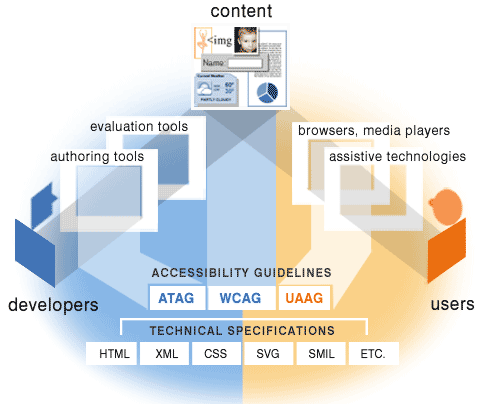
\includegraphics[width=9cm]{figs/accesibilidad.png}
\end{center}


\begin{flushright}
{\tiny
Source: \url{http://www.w3.org/WAI/intro/specs}
}
\end{flushright}

\end{frame}


 % grex

% ST, jgb, 2022-03-24
% SARO, jgb, 2022-03-24
%
%

%%-----------------------------------------------------
%%-----------------------------------------------------
\usebackgroundtemplate{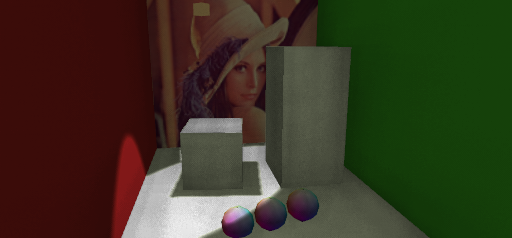
\includegraphics[width=\paperwidth,height=\paperheight]{figs/webgl-cornellbox}}
% Original figure: ``3D image of Cornell Box scene made with WebGL''
% from StormEngineC 3D Library
% License:  GNU Free Documentation License, Version 1.2 or later
% https://commons.wikimedia.org/wiki/File:WebGL_Cornell_Box.png
{\bf
  \textcolor[rgb]{1,1,1}{
    \section{Navegar en tres dimensiones}
  }
}

\usebackgroundtemplate{}

%%-----------------------------------------------------
\begin{frame}
\frametitle{WebGL}

\begin{columns}[T]
  \begin{column}{.40\textwidth}
    
\includegraphics[width=5.5cm]{figs/webgl-logo}
    \vspace{2cm}
    {\Large
      Mantenido por el Khronos Group
    }
  \end{column}%
  \hfill%
  \begin{column}{.58\textwidth}
    {\Large
      \begin{itemize}
      \item API JavaScript para gráficos interactivos en 3D
      \item Primeros desarrollos por Mozilla
      \item Proporcionada por los principales navegadores
      \item Puede mezclarse con HTML
      \item Basado en OpenGL
      \end{itemize}
    }
  \end{column}%
\end{columns}

\end{frame}

%%-----------------------------------------------------
\begin{frame}
\frametitle{Bibliotecas y utilidades}

{\Large
\begin{itemize}
\item API alto nivel: three.js, babylon.js
\item Motores de juegos: Unreal 4, Unity 5
\item Creación de escenas: Blender con Blend4Web, Clara.io
\end{itemize}
}
\vspace{1cm}
\begin{flushright}
  \url{http://threejs.org/} \\
  \url{http://babylonjs.com/} \\
  \url{https://blend4web.com/} \\
\end{flushright}
\end{frame}

%%-----------------------------------------------------
\begin{frame}
\frametitle{Algunos ejemplos}

{\Large
  \begin{itemize}
    \item Cube \\
    \url{http://www.playmapscube.com/} \\
  \item Experience Curiosity (Blend4Web)\\
    \url{http://eyes.nasa.gov/curiosity/} \\
  \item Sponza demo (babylon.js) \\
    \url{http://www.babylonjs.com/Demos/Sponza/} \\
  \item Above the clouds (three.js) \\
    \url{http://earth.plus360degrees.com/} \\
  \end{itemize}
}

\end{frame}


%%-----------------------------------------------------
\begin{frame}
\frametitle{Referencias y enlaces}

\begin{flushright}
  WebGL en Wikipedia \\
  \url{https://en.wikipedia.org/wiki/WebGL} \\
  \vspace{.5cm}
  WebGL en Mozilla Developer Network \\
  \url{https://developer.mozilla.org/en-US/docs/Web/API/WebGL_API} \\
  \vspace{.5cm}
  ``3D image of Cornell Box scene made with WebGL'', \\
  from StormEngineC 3D Library, GFDL 1.2 \\
  \url{https://commons.wikimedia.org/wiki/File:WebGL_Cornell_Box.png} \\
  \vspace{.5cm}
  ``WebGL tutorial'', by Mozilla \\
  \url{https://developer.mozilla.org/en-US/docs/Web/API/WebGL_API/Tutorial} \\
\end{flushright}  

\end{frame}






 % jgb
\section{Scalable Vector Graphics}

%-----------------------    ---------------------------------

\begin{frame}
\frametitle{¿Qué es SVG?}

\begin{itemize}
   \item SVG es vectorial
   \item Apto para iconos e imágenes de alta calidad
   \item Puede ampliarse o reducirse sin perder calidad (esencial para la \emph{responsive web}
   \item ermite optimización gracias a la \emph{caché} de recursos gráficos
   \item Los navegadores modernos ofrecen soporte SVG nativo
\end{itemize}

\end{frame}


%-----------------------    ---------------------------------

\begin{frame}
\frametitle{El porqué de SVG visualmente}

\begin{center}
  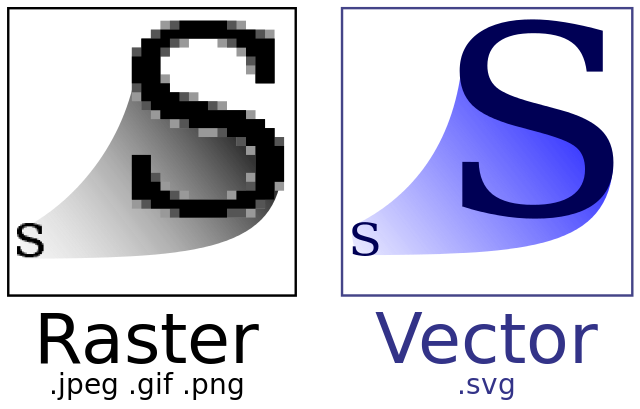
\includegraphics[width=10cm]{figs/svg.png}
\end{center}


\begin{flushright}
{\tiny
Source: https://commons.wikimedia.org/wiki/File:Bitmap\_VS\_SVG.svg
}
\end{flushright}

\end{frame}

%-----------------------    ---------------------------------

\begin{frame}
\frametitle{SVG}

\begin{itemize}
   \item SVG es un estándar basado en XML del W3C
   \item Permite tres tipos de objetos gráficos:
   \begin{itemize}
     \item Elementos geométricos vectoriales (p.e. caminos consistentes en rectas y curvas, y áreas limitadas por ellos)
     \item Imágenes de mapa de bits /digitales
     \item Texto
   \end{itemize}
   \item Existe un validador del W3C
   \item Hay múltiples herramientas para manipular SVGs: Inkscape, Adobe Illustrator, ...
\end{itemize}

\end{frame}

%-----------------------    ---------------------------------

\begin{frame}[fragile]
\frametitle{Ejemplo de SVG}

Un ejemplo con SVG:

\begin{footnotesize}
\begin{verbatim}
<svg xmlns="http://www.w3.org/2000/svg" version="1.1">
  <rect x="25" y="25" width="200" height="200" fill="lime"
        stroke-width="4" stroke="pink" />
  <circle cx="125" cy="125" r="75" fill="orange" />
  <polyline points="50,150 50,200 200,200 200,100" stroke="red" 
            stroke-width="4" fill="none" />
  <line x1="50" y1="50" x2="200" y2="200" stroke="blue" 
        stroke-width="4" />
</svg>
\end{verbatim}
\end{footnotesize}

\end{frame}

%-----------------------    ---------------------------------

\begin{frame}
\frametitle{Resultado visual}

\begin{center}
  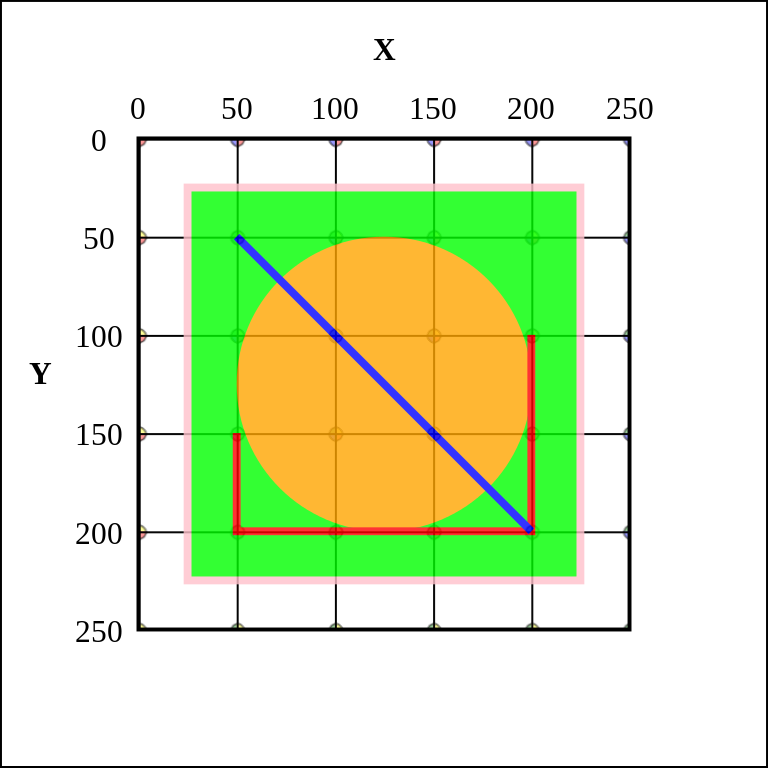
\includegraphics[width=7cm]{figs/svg-example.png}
\end{center}

\begin{flushright}
{\tiny
Source: https://commons.wikimedia.org/wiki/File:SVG\_example\_markup\_grid.svg
}
\end{flushright}

\end{frame}

 % grex
%
%

%%-----------------------------------------------------
%%-----------------------------------------------------
\section{Viéndose con gente...}

%%-----------------------------------------------------
\begin{frame}
\frametitle{Meetup}

\begin{columns}[T]
\begin{column}{.48\textwidth}
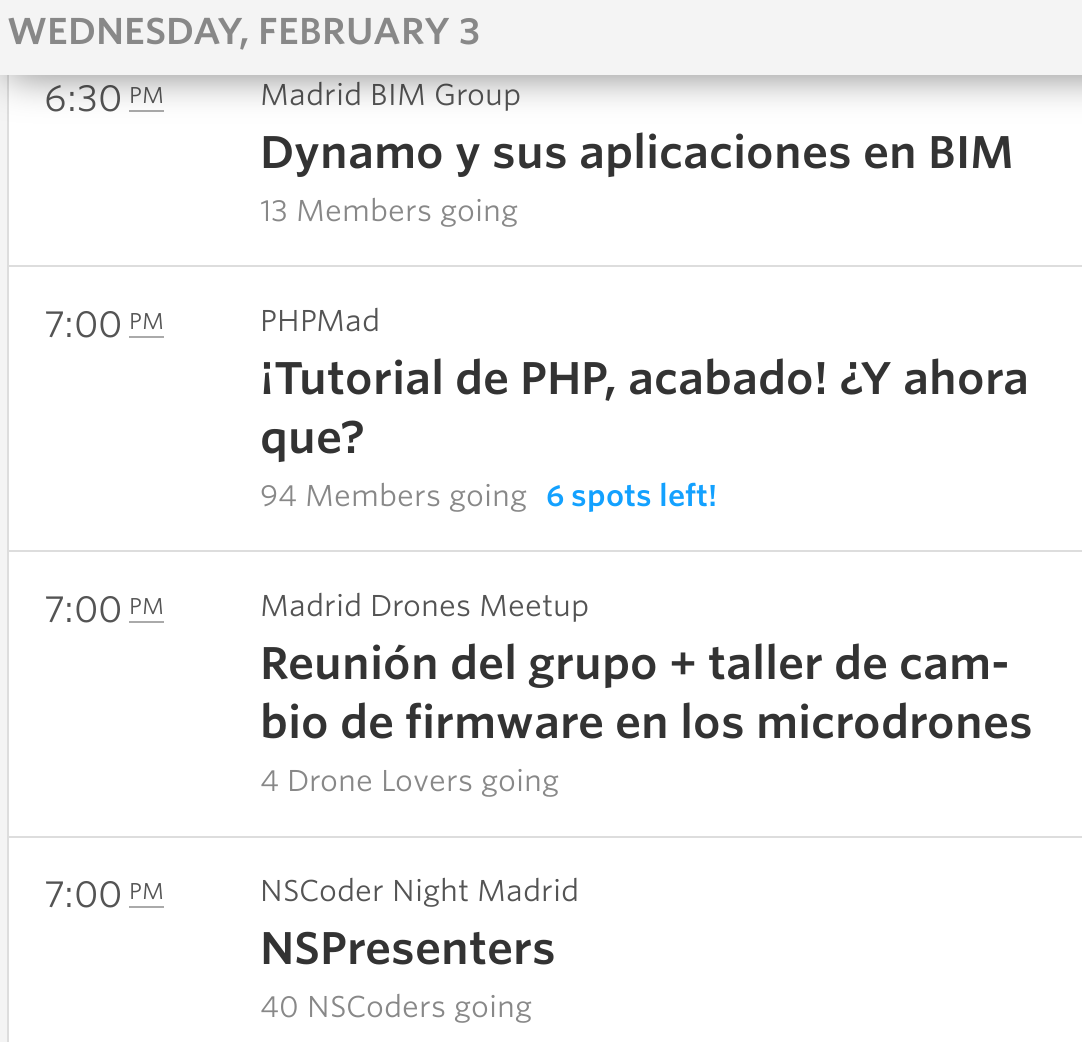
\includegraphics[width=6.5cm]{figs/meetup-calendar}

\begin{flushright}
  {\Large
    \url{http://meetup.com}
  }
\end{flushright}

\end{column}%
\hfill%
\begin{column}{.50\textwidth}
  \begin{flushright}
    
\includegraphics[width=5cm]{figs/meetup-logo}
  \end{flushright}
{\Large
\begin{itemize}
\item Información sobre reuniones cercanas
\item Mucho contenido ténico
\item Y mucho que no
\end{itemize}
}
\end{column}%
\end{columns}

\end{frame}

%%-----------------------------------------------------
\begin{frame}
\frametitle{Grupos}

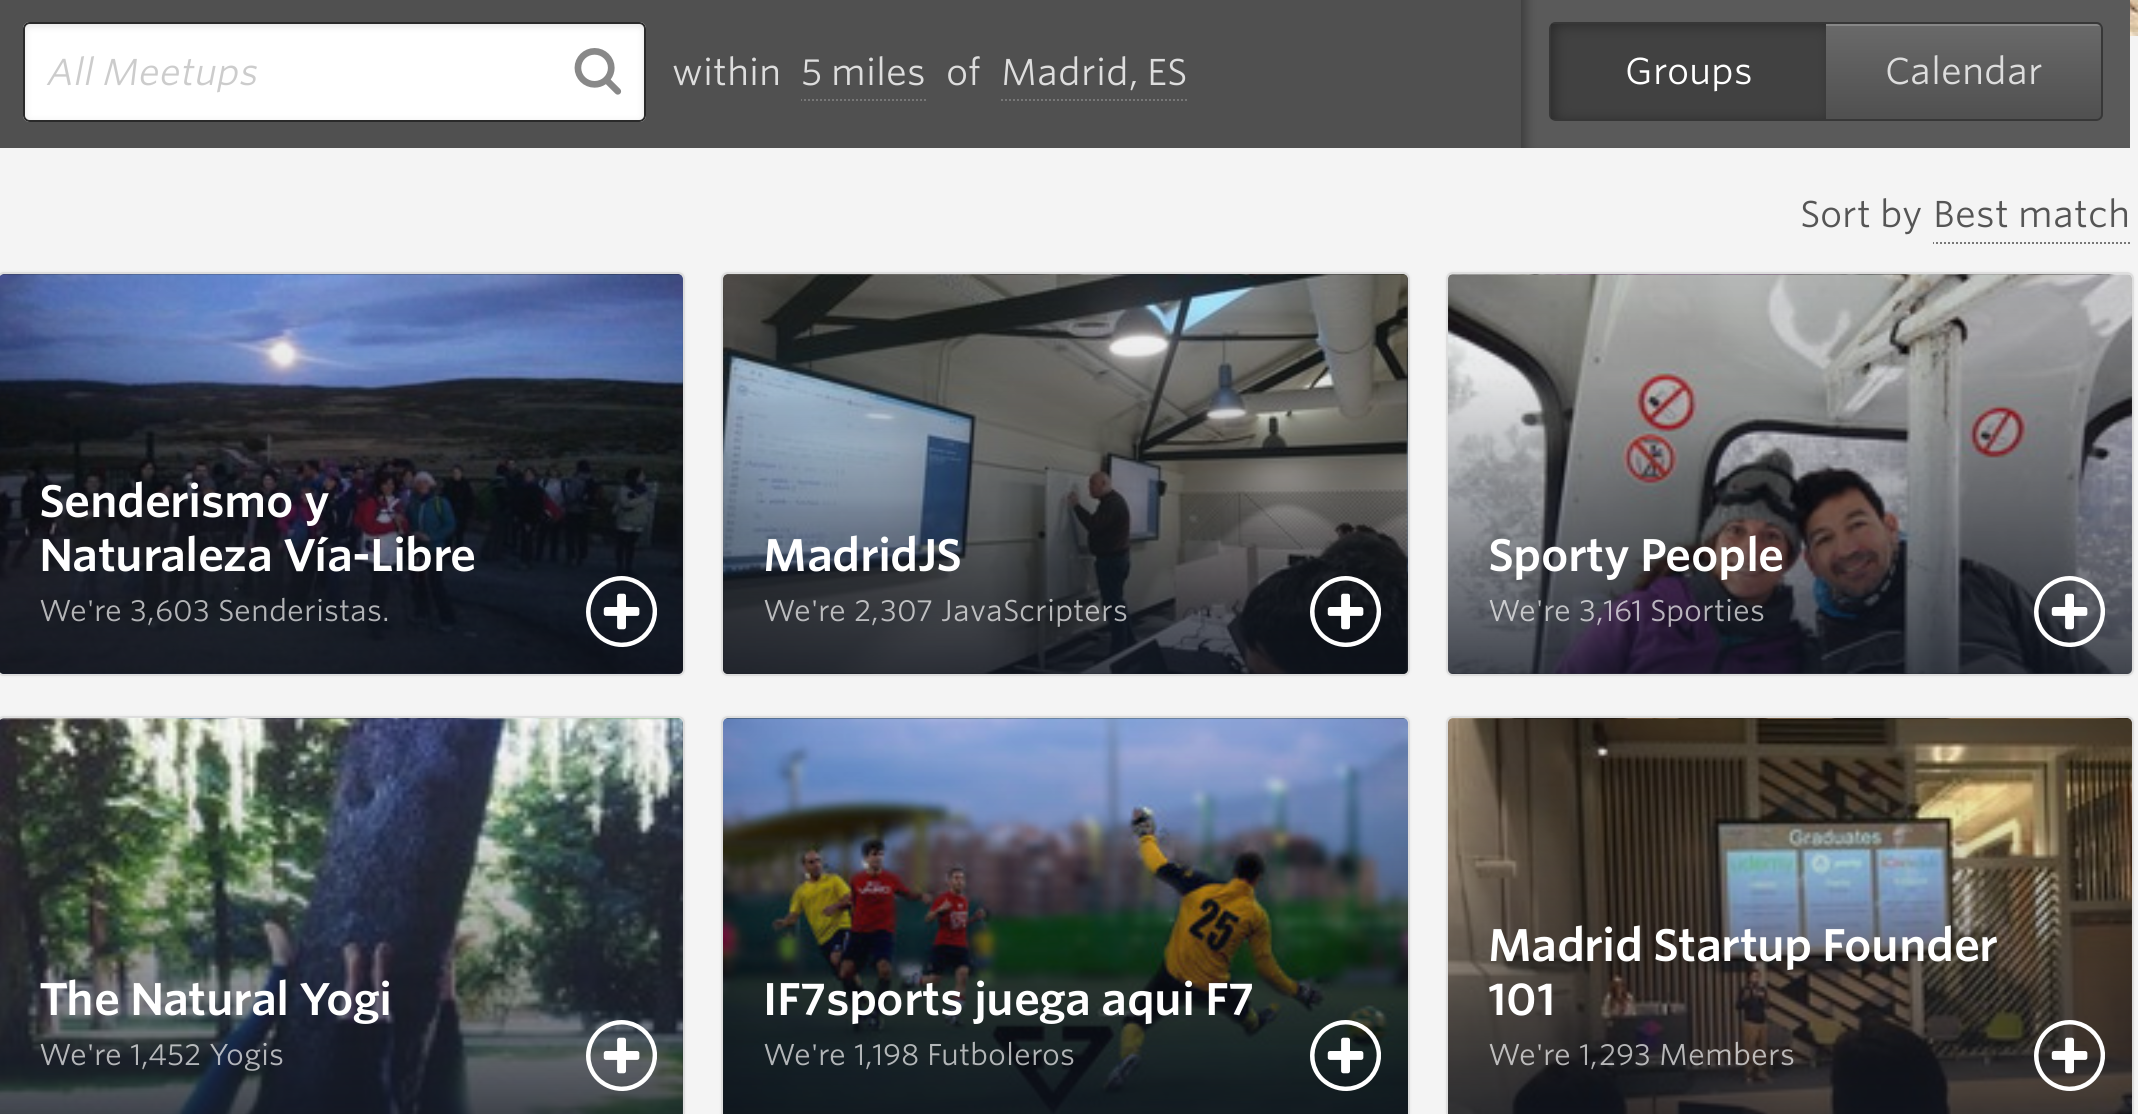
\includegraphics[width=11.5cm]{figs/meetup-near-madrid} 

\end{frame}

%%-----------------------------------------------------
\begin{frame}
\frametitle{Reuniones}

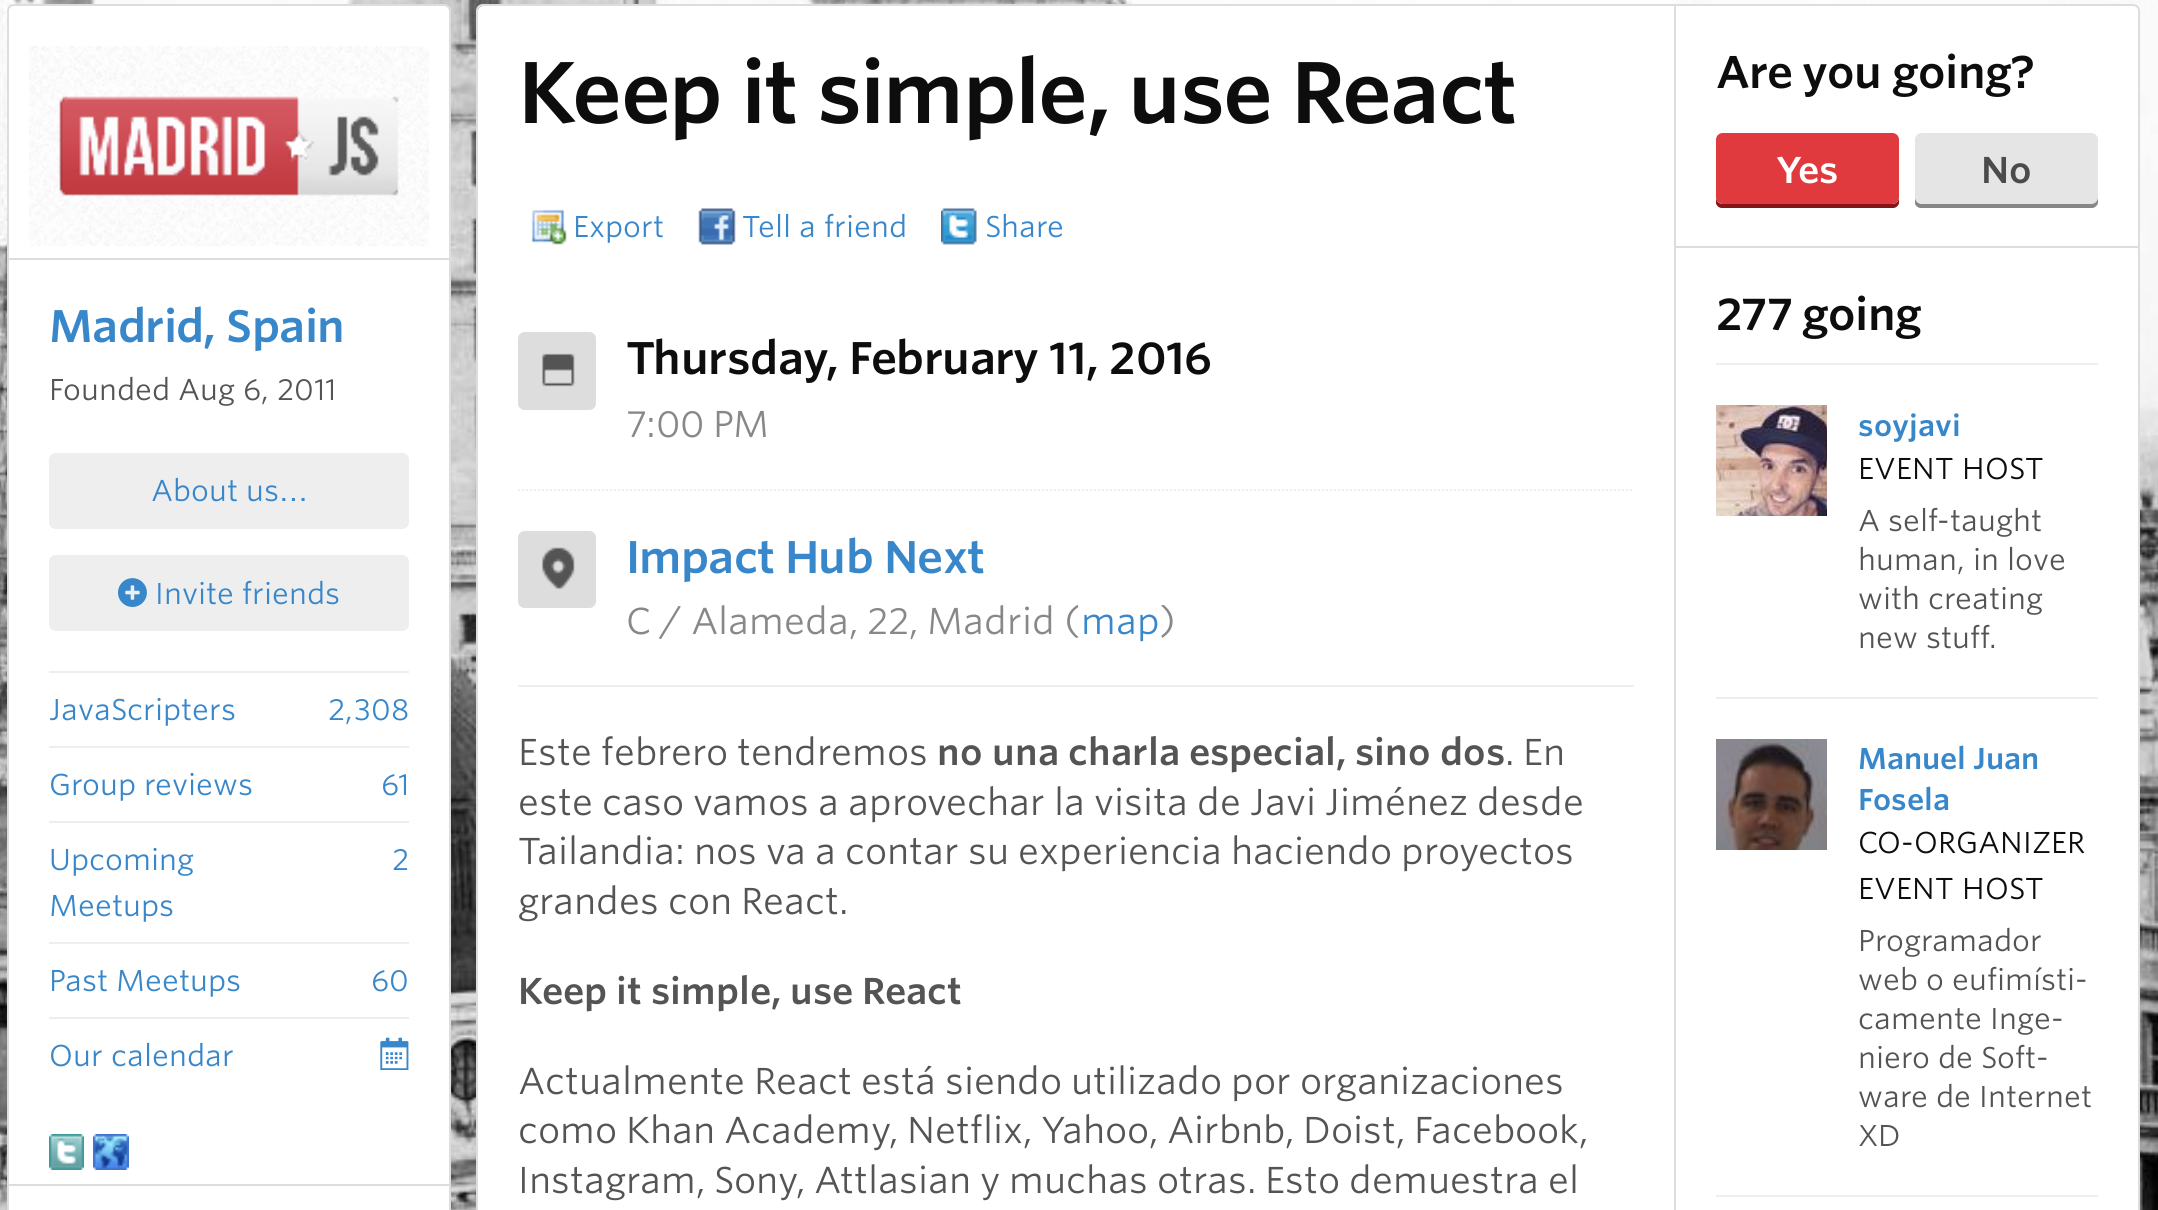
\includegraphics[width=11.5cm]{figs/meetup-meeting} 

\end{frame}






 % jgb

% ST, jgb, 2022-04-07
% SARO, jgb, 2022-04-07
\include{browsers-history} % jgb
%%
%

%%-----------------------------------------------------
%%-----------------------------------------------------
\section{Localizando a quien se deje}

%%-----------------------------------------------------
\begin{frame}
\frametitle{Escenario}

{\Large
Queremos saber quien está en nuestro edificio:

\begin{itemize}
\item Con el mínimo esfuerzo nuestro posible.
\item Con el mínimo esfuerzo por parte de quienes están en el edificio.
\itme Pero podemos suponer una colaboración por su parte \\
(están interesados en que se sepa que están).
\item El edificio no es muy grande, y está aislado.
\item Una solución aproximada es suficiente.
\end{itemize}
}

{\huge
\begin{center}
¿Ideas?
\end{center}
}
\end{frame}

%%-----------------------------------------------------
\begin{frame}
\frametitle{¿Y si usamos WiFi?}

{\Large
\begin{itemize}
\item Casi todos llevan teléfono
\item Casi todos llevan WiFi activado
\item Cada teléfono usa una MAC WiFi distinta
\item Podemos pedir un registro de MACs (app web simple)
\end{itemize}
}

\vspace{1cm}

{\huge
\begin{center}
¿Cómo sabemos quién está en el edificio?
\end{center}
}

\end{frame}

%%-----------------------------------------------------
\begin{frame}
\frametitle{Detectando MACs en nuestra red WiFi}

{\Large

\begin{itemize}
\item Si somos el punto de acceso (AP), sabemos todas las MAC conectadas
\item Si escuchamos en un canal, recibimos todas las MAC que emiten
\item Pero la electrónica y el software tienen que permitirlo
\end{itemize}
}

El caso de Android:

\begin{itemize}
\item Si tenemos acceso root (eg, CyanogenMod), tenemos un kernel Linux.
\item La electrónica y el software permiten modo AP.
\item Podemos ver todo lo que ve el kernel
\item De hecho, para muchas cosas no hace falta estar en modo AP.
\end{itemize}

\begin{flushright}
{\small
  \url{https://github.com/rorist/android-network-discovery}
}
\end{flushright}
\end{frame}
 % jgb
%%
%

%%-----------------------------------------------------
%%-----------------------------------------------------
\section{¿Cómo sabe mi navegador dónde estoy?}

%%-----------------------------------------------------
\begin{frame}
\frametitle{Pero qué listo es tu móvil}

{\Large
Vete a un sitio donde no haya cobertura GPS

\begin{flushright}
o deshabilita el GPS de tu móvil
\end{flushright}

Lanza la aplicación Google Maps

\begin{flushright}
O busca tu localización en OpenStreetMap

\url{http://www.openstreetmap.org}
\end{flushright}
}

{\huge
\begin{center}
¿Cómo es posible?
\end{center}
}
\end{frame}

%%-----------------------------------------------------
\begin{frame}
\frametitle{Servicios de localización}

{\Large
Bases de datos con coordenadas de puntos de medida de:

\begin{itemize}
\item potencia recibida de puntos de acceso WiFi (MAC, SSID)
\item potencia recibida de estaciones base de redes móviles (CellID)
\end{itemize}

También pueden incluir geolocalización de direcciones IP

\begin{flushright}
\url{http://en.wikipedia.org/wiki/Wi-Fi_positioning_system}
\end{flushright}
}

\end{frame}


%%-----------------------------------------------------
\begin{frame}
\frametitle{Uso de servicios de localización}

{\Large
Ejemplo: Google Play Location Services \\
}
\begin{flushright}
\url{https://developer.android.com/google/play-services/location.html}
\end{flushright}

{\Large
Ejemplo: API JavaScript de Firefox \\
}

\begin{flushright}
\url{https://www.mozilla.org/en-US/firefox/geolocation/} \\
\url{https://developer.mozilla.org/en-US/docs/Web/API/Geolocation/Using_geolocation}
\end{flushright}
\end{frame}

%%-----------------------------------------------------
\begin{frame}
\frametitle{Mozilla Location Service y Stumbler}

\includegraphics[height=6cm]{figs/mozilla-location-map}

\begin{flushright}
  \url{https://location.services.mozilla.com/map} \\
  \url{https://location.services.mozilla.com/} \\
\end{flushright}
\end{frame}

%%-----------------------------------------------------
\begin{frame}
\frametitle{OpenCellID}

\includegraphics[height=6cm]{figs/opencellid-map}

\begin{flushright}
  \url{http://opencellid.org/} \\
  \url{http://wiki.opencellid.org/wiki/What_is_OpenCellID} \\
  \url{http://wiki.opencellid.org/wiki/Data_sources} \\
\end{flushright}
\end{frame}
 % jgb
%
\section{Raspberry Pi}

\begin{frame}
\frametitle{Raspberry Pi}

\begin{center}
  \includegraphics[width=10cm]{figs/raspberry.jpg}
\end{center}


\begin{flushright}
{\tiny
Source: Wikipedia
}
\end{flushright}

\end{frame}

%-----------------------    ---------------------------------

\begin{frame}
\frametitle{¿Qué es la Raspberry Pi?}

\begin{itemize}
   \item Ideada para educación; para entender cómo funciona la computación
   \item Es una placa de ordenador del tamaño de una tarjeta de crédito
   \item Cuesta 35 euros (sólo la placa)
   \item Muchos accesorios (incluidas cajas)
   \item Cuenta con sistemas operativos específicos
   \item El sistema operativo va en una tarjeta microSD
   \item Muchos proyectos \emph{maker}: sistema multimedia casero, servidor web,
\emph{router}, y muchos más.
\end{itemize}

\end{frame}


%-----------------------    ---------------------------------

\begin{frame}
\frametitle{Raspberry Pi: Puertos}

\begin{center}
  \includegraphics[width=11cm]{figs/raspberry2.jpg}
\end{center}


\begin{flushright}
{\tiny
(cc) Phil Sheard (from Flickr)
}
\end{flushright}

\end{frame}



%

%%-----------------------------------------------------
%%-----------------------------------------------------
\section{SSH: Trabajando desde remoto}


%-----------------------    ---------------------------------

\begin{frame}
\frametitle{�Qu� es SSH?}

\begin{itemize}
   \item Permite abrir terminales remotos
   \item La informaci�n va cifrada
   \item M�quinas de los laboratorios del GSyC
   \begin{itemize}
     \item Parte de guerra: http://sherlock.gsyc.es/parte\_de\_guerra/
   \end{itemize}
   \item \texttt{scp} permite copiar ficheros remotos
   \item Hay cliente para Windows: \texttt{PuTTY}
   \item Permite crear \emph{t�neles}
\end{itemize}

\end{frame}


%-----------------------    ---------------------------------

\begin{frame}
\frametitle{SSH en acci�n}

\begin{center}
  \includegraphics[width=10cm]{figs/terminal.png}
\end{center}


\begin{flushright}
{\tiny
Source: http://carina.org.uk/guidepics/terminal1.png
}
\end{flushright}

\end{frame}



%-----------------------    ---------------------------------

\begin{frame}
\frametitle{SSH}

\begin{center}
  \includegraphics[width=10cm]{figs/ssh-tunnel.png}
\end{center}


\begin{flushright}
{\tiny
Source: http://www.codemastershawn.com/library/tutorial/images/ssh.tunnel.overview.gif
}
\end{flushright}

\end{frame}




%%%-----------------------------------------------------
%%-----------------------------------------------------
\section{Scratch: Enseña a programar}


%-----------------------    ---------------------------------


\begin{frame}
\frametitle{}

\begin{center}
  \includegraphics[width=8cm]{figs/scratch.jpg}
\end{center}


\begin{flushright}
{\tiny
http://canaltic.com/vr/manual/scratch001.jpg
}
\end{flushright}

\end{frame}


%-----------------------    ---------------------------------

\begin{frame}
\frametitle{Scratch y AppInventor}

\begin{itemize}
   \item Fruto de la preocupación de falta de interés por la programación
   \item Es un subconjunto de lo que se conoce como potenciaciación del pensamiento computacional
   \item Hay 10 veces más líneas de código en un coche (de gama alta, hoy) que en un avión
   \item Programación visual, orientada a la enseñanza
   \item Las plataformas permiten compartir y remezclar
\end{itemize}

\end{frame}



%-----------------------    ---------------------------------

\begin{frame}
\frametitle{}

\begin{center}
  \includegraphics[width=10cm]{figs/appInventor.png}
\end{center}


\begin{flushright}
{\tiny
http://www.carloslabs.com/files/app-inventor/accelerometer-test.gif
}
\end{flushright}

\end{frame}



%\section{Google Cardboard}
%-----------------------    ---------------------------------

\begin{frame}
\frametitle{Google Cardboard}

\begin{center}
  \includegraphics[width=9cm]{figs/google-cardboard.jpg}
\end{center}


\begin{flushright}
{\tiny
Source: http://images.techtimes.com/data/images/full/10137/google-cardboard.jpg
}
\end{flushright}

\end{frame}


%-----------------------    ---------------------------------

\begin{frame}
\frametitle{Google Cardboard}

\begin{center}
  \includegraphics[width=8cm]{figs/google-cardboard2.jpg}
\end{center}


\begin{flushright}
{\tiny
Source: http://uploads.webflow.com/53acec028f16901b3d5ca6c1/53acec104f02f4e04bcd4ec5\_1.png
}
\end{flushright}

\end{frame}


%-----------------------    ---------------------------------

\begin{frame}
\frametitle{¿Qué es el Google Cardboard?}

\begin{itemize}
   \item Experimenta realidad virtual de manera sencilla y barata (19 euros)
   \item Cuesta 35\% (aunque hay instrucciones para hacerla tú mismo con una caja de pizza)
   \item Hay varias aplicaciones en el Google Play: cardboard, etc.
   \item API en Java
   \item También se pueden utilizar extensiones de Chrome escritas en Javascript (con Tree.js)
\end{itemize}

\end{frame}


%-----------------------    ---------------------------------

\begin{frame}
\frametitle{Google Cardboard ``ingredients''}

\begin{center}
  \includegraphics[width=11cm]{figs/ingredients.png}
\end{center}


\begin{flushright}
{\tiny
Source: https://cardboard.withgoogle.com/
}
\end{flushright}

\end{frame}



%\include{heartbleed} % jgb
%%
%

%%-----------------------------------------------------
%%-----------------------------------------------------
\section{En las nubes}

%%-----------------------------------------------------
\begin{frame}
\frametitle{OpenStack}

\begin{columns}[T]
\begin{column}{.38\textwidth}
\includegraphics[width=6.5cm]{figs/openstack-logo}

\begin{flushright}
\url{http://openstack.org}
\end{flushright}

\end{column}%
\hfill%
\begin{column}{.60\textwidth}
{\Large
\begin{itemize}
\item Plataforma para la computación en nube
\item Software libre
\item Tecnología básica: \\
  Python / Django
\item Gestión vía línea de comandos, \\
  API REST, dashboard
\item Inicio: 2010 \\
  (NASA, Rackspace)
\item Gestionado por la \\
  OpenStack Foundation
\end{itemize}
}
\end{column}%
\end{columns}

\end{frame}

%%-----------------------------------------------------
\begin{frame}
\frametitle{Principales components}

\begin{columns}[T]
\begin{column}{.45\textwidth}
{\Large
\begin{itemize}
\item Computación
\item Almacenamiento de objetos
\item Almacenamiento de bloques
\item Red
\item Dashboard
\end{itemize}
}
\end{column}%
\hfill%
\begin{column}{.45\textwidth}
{\Large
\begin{itemize}
\item Servicio de identidades
\item Servicio de imágenes
\item Telemetría
\item Orquestación
\item Base de datos
\item Metal desnudo
\end{itemize}
}
\end{column}%
\end{columns}

\end{frame}

%%-----------------------------------------------------
\begin{frame}
\frametitle{Horizon: el dashboard}

\includegraphics[height=7cm]{figs/openstack-screenshot}

\begin{flushright}
\url{https://www.youtube.com/watch?v=TgPTjrf1y0A}
\end{flushright}

\end{frame}

%%-----------------------------------------------------
\begin{frame}
\frametitle{Las empresas}

\begin{columns}[T]
\begin{column}{.55\textwidth}
\includegraphics[width=6.5cm]{figs/openstack-platinum}\\
\vspace{1cm}
\includegraphics[width=6.5cm]{figs/openstack-gold}\\
\end{column}%
\hfill%
\begin{column}{.41\textwidth}
\includegraphics[width=4.5cm]{figs/openstack-silver}
\end{column}%
\end{columns}

\end{frame}





 % jgb
%%
%

%%-----------------------------------------------------
%%-----------------------------------------------------
\section{Tres son multitud...}

%%-----------------------------------------------------
\begin{frame}
\frametitle{Los ataques ``man in the middle''}

\begin{columns}[T]
\begin{column}{.48\textwidth}
\includegraphics[width=6.5cm]{figs/man-in-the-middle}


\end{column}%
\hfill%
\begin{column}{.48\textwidth}
{\Large
\begin{itemize}
\item Monitorizar o alterar una comunicación.
\item Trivial en HTTP (texto claro).
\item HTTPS (TLS/SSL): \\
  Cifrado y certificados para evitarlo.
\end{itemize}
}
\end{column}%
\end{columns}
\vspace{1cm}
\begin{flushright}
{\footnotesize
Imagen ``Man in the Middle'', by Martial Régereau, CC by-sa 3.0 \\
\url{http://commons.wikimedia.org/wiki/File:Attaque_Man_In_The_Middle.jpg} 
}
\end{flushright}

\end{frame}

%%-----------------------------------------------------
\begin{frame}
\frametitle{Lenovo, Superfish y Komodia}

{\large
\begin{itemize}
\item Lenovo instala Superfish en varios modelos (octubre-diciembre 2014)
\item Se descubre que Superfish realiza ataque \\
  ``man in the middle'' para inyectar publicidad \\
\item Superfish instala un certificado de CA raíz, \\
  y establece un proxy para HTTP/HTTPS \\
\item Tecnología de Komodia, se usa en muchos sistemas (redes de empresas, software de control parental, etc.)
\item Al menos en algunos de ellos se han demostrado ataques ``man in the middle'' por terceras partes.
\end{itemize}
}

\begin{flushright}
{\footnotesize
\url{http://www.forbes.com/sites/thomasbrewster/2015/02/19/superfish-need-to-know/} \\
\url{http://arstechnica.com/security/2015/02/ssl-hijacker-behind-superfish-debacle-imperils-big-number-of-users/} \\
}
\end{flushright}
\end{frame}

%%-----------------------------------------------------
\begin{frame}
\frametitle{¿Cómo actúa Superfish en los Lenovo?}

{\Large
\begin{itemize}
\item Configura proxy para comunicación del navegador.
\item Instala un certificado de CA raíz propia.
\item Conexiones HTTPS ``capturadas'' por proxy.
\item De navegador a proxy, SSL con certificado firmado por la propia CA.
\item De proxy a sitio, SSL con certificado real.
\item Proxy: toda la comunicación en claro.
\item Certificados generados al vuelo: \\
  necesaria la clave privada de la nueva CA. \\
\item Resumen: terceros pueden leer conexiones HTTPS.
\end{itemize}
}

\begin{flushright}
{\footnotesize
\url{https://nakedsecurity.sophos.com/2015/02/20/the-lenovo-superfish-controversy-what-you-need-to-know/} \\
\url{http://blog.erratasec.com/2015/02/exploiting-superfish-certificate.html} \\
}
\end{flushright}
\end{frame}
 % jgb
%
\section{Google Chromecast}

%-----------------------    ---------------------------------

\begin{frame}
\frametitle{Google Chromecast}

\begin{center}
  \includegraphics[width=10cm]{figs/chromecast.jpg}
\end{center}


\begin{flushright}
{\tiny
Source: Wikipedia
}
\end{flushright}

\end{frame}



%-----------------------    ---------------------------------

\begin{frame}
\frametitle{Google Chromecast conectado}

\begin{center}
  \includegraphics[width=10cm]{figs/enlatele.jpg}
\end{center}


\begin{flushright}
{\tiny
Source: Wikipedia
}
\end{flushright}

\end{frame}



%-----------------------    ---------------------------------

\begin{frame}
\frametitle{¿Qué es Chromecast?}

\begin{itemize}
   \item Permite convertir tu TV en un \emph{smart TV}
   \item Se maneja desde un dispositivo móvil
   \item Las aplicaciones pueden tener soporte para Chromecast
   \item Se conecta al puerto HDMI de la TV y la wifi
   \item Permite hacer \emph{streaming}
   \item Cuesta 35 euros
   \item Programable mediante SDK propio
\end{itemize}

\end{frame}


%-----------------------    ---------------------------------

\begin{frame}
\frametitle{Tu móvil en la TV}

\begin{center}
  \includegraphics[width=10cm]{figs/mirror.png}
\end{center}


\begin{flushright}
{\tiny
Source: Google
}
\end{flushright}

\end{frame}



%\section{\LaTeX}

%-----------------------    ---------------------------------

\begin{frame}
\frametitle{¿Qué es \LaTeX ?}

\begin{itemize}
   \item Sistema de composición de textos
   \item \LaTeX\ en realidad es un conjunto de scripts para facilitar el uso del lenguaje de composición tipográfica \TeX\ creado por Donald Knuth
   \item No es WYSIWYG, sino que se basa en instrucciones
   \item Se compila, para obtener el resultado final (generalmente, un PDF)
   \item (aunque hay editores \LaTeX\ WYSIWG, como LyX)
   \item Ventajas:
   \begin{itemize}
     \item Separa visualización de contenido
     \item Gestión de referencias (a figuras, tablas, capítulos...)
     \item Tablas de contenidos, figuras y tablas generada automáticamente
     \item Gestión bibliográfica
     \item Fórmulas matemáticas, caracteres especiales...
     \item Es texto plano... ideal para \texttt{grep} y \texttt{GitHub}
   \end{itemize}
\end{itemize}

\end{frame}

%-----------------------    ---------------------------------

\begin{frame}
\frametitle{¿Para qué se utiliza \LaTeX ?}

\begin{itemize}
   \item Se utiliza mucho en textos científico técnicos
   \item Por ejemplo, puedes utilizarlo para escribir la memoria de tu Trabajo Fin de Grado. Tienes una plantilla disponible en \url{https://github.com/gregoriorobles/plantilla-memoria}
   \item En GSyC las utilizamos para nuestras transparencias (¡Estas transparencias están hechas en \LaTeX\ (con Beamer)!)
\end{itemize}

\end{frame}


%-----------------------    ---------------------------------

\begin{frame}
\frametitle{Flujo de trabajo en \LaTeX}

\begin{center}
  \includegraphics[width=8cm]{figs/latex.png}
\end{center}


\begin{flushright}
{\tiny
Fuente: Wikipedia (Creative Commons Attribution-ShareAlike)
}
\end{flushright}

\end{frame}



%\section{DShell - Análisis forense en redes}

%-----------------------    ---------------------------------

\begin{frame}
\frametitle{¿Qué es Dshell? ¿Y el análisis forense?}

\begin{itemize}
   \item Es un \emph{framework} de análisis forense en redes
   \item (Análisis forense: \emph {aplicación de técnicas científicas y analíticas especializadas a infraestructura tecnológica que permiten identificar, preservar, analizar y presentar datos que sean válidos dentro de un proceso legal.} \texttt{WikiPedia})
   \item Desarrollado por la U.S. Army
   \item Está en GitHub: \url{https://github.com/USArmyResearchLab/Dshell}
\end{itemize}

\end{frame}


%-----------------------    ---------------------------------

\begin{frame}
\frametitle{¿Para qué el análisis forense?}

\begin{itemize}
   \item La seguridad informática (especialmente en redes) es un tema que está siendo muy trabajado últimamente
   \item Wireshark es un analizador de tráfico visual, limitado para análisis forense
   \item Existen múltiples ataques
   \item Existen múltiples herramientas para atajar el problema
\end{itemize}

\end{frame}

%-----------------------    ---------------------------------

\begin{frame}
\frametitle{Dshell es una herramienta de la U.S. Army}

\begin{center}
  \includegraphics[width=10cm]{figs/dshell}
\end{center}


\begin{flushright}
{\tiny
Source: http://www.army.mil/media/379387/
}
\end{flushright}

\end{frame}



%-----------------------    ---------------------------------

\begin{frame}
\frametitle{No estás solo en Internet}

Posibles riesgos:

\begin{itemize}
  \item Pasivos
    \begin{itemize}
      \item wiretapping
      \item Port scanner
      \item Idle scan
    \end{itemize}
  \item Active
    \begin{itemize}
      \item Denial-of-service attack
      \item DNS spoofing
      \item Spoofing
      \item Man in the middle
      \item ARP poisoning
      \item Smurf attack
      \item Buffer overflow
      \item Heap overflow
      \item Format string attack
      \item SQL injection
      \item Cyber-attack
    \end{itemize}   
\end{itemize}

\end{frame}




%%
%

%%-----------------------------------------------------
%%-----------------------------------------------------
\section{Libros libres}

%%-----------------------------------------------------
\begin{frame}
\frametitle{Proyecto Gutenberg}

\begin{columns}[T]
\begin{column}{.38\textwidth}
\includegraphics[width=5.5cm]{figs/gutenberg-logo}

\begin{flushright}
{\small
\url{http://gutenberg.org/}
}
\end{flushright}

\end{column}%
\hfill%
\begin{column}{.60\textwidth}
{\Large
\begin{itemize}
\item Biblioteca de libros libres
\item Normalmente, derechos de autor expirados
\item Digitalizados y corregidos por voluntarios
\item También hay audiolibros \\
  leidos por voluntarios
\item Abril de 2015: 46,000 libros \\
  (100,000 incluyendo proyectos afiliados)
\end{itemize}
}
\end{column}%
\end{columns}

\end{frame}

%%-----------------------------------------------------
\begin{frame}
\frametitle{Ejemplo de libro}

\includegraphics[width=10.cm]{figs/gutenberg-book}

\begin{flushright}
{\small
\url{http://www.gutenberg.org/ebooks/98}
}
\end{flushright}
\end{frame}

%%-----------------------------------------------------
\begin{frame}
\frametitle{No sólo en inglés}

\includegraphics[width=12.cm]{figs/gutenberg-quijote}

\begin{flushright}
{\small
\url{http://www.gutenberg.org/ebooks/2000}
}
\end{flushright}
\end{frame}

%%-----------------------------------------------------
\begin{frame}
\frametitle{Proyectos relacionados}

{\Large

\begin{itemize}
\item Distributed Proofreaders \\
  \url{http://pgdp.net}
\item LibriVox: audiolibros (leidos por voluntarios) \\
  \url{http://librivox.org}
\item Wikibooks: Libros de texto ``estilo wiki''\\
  \url{http://en.wikibooks.org}
\item Cervantes Virtual: Libros en español \\
  \url{http://www.cervantesvirtual.com}
\item Europeana: artículos ``culturales'' \\
  \url{http://www.europeana.eu}
\end{itemize}

}

\end{frame}



%%
%

%%-----------------------------------------------------
%%-----------------------------------------------------
\section{Analiza que algo queda}

%%-----------------------------------------------------
\begin{frame}
\frametitle{OpenHub}

\begin{center}
\includegraphics[width=10cm]{figs/analisis-openhub}
\end{center}

\begin{flushright}
\url{https://openhub.net}
\end{flushright}

\end{frame}

%%-----------------------------------------------------
\begin{frame}
\frametitle{OpenHub (2)}

\begin{center}
\includegraphics[width=11cm]{figs/analisis-openhub-2}
\end{center}

\end{frame}

%%-----------------------------------------------------
\begin{frame}
\frametitle{GitHub Pulse}

\begin{center}
\includegraphics[width=10.5cm]{figs/analisis-github}
\end{center}

\begin{flushright}
\url{https://github.com}
\end{flushright}

\end{frame}

%%-----------------------------------------------------
\begin{frame}
\frametitle{GitHub Charts}

\begin{center}
\includegraphics[width=12cm]{figs/analisis-github-2}
\end{center}

\end{frame}
 % jgb
%

%%-----------------------------------------------------
%%-----------------------------------------------------
\section{Navegando sin bloqueos IP}


%-----------------------    ---------------------------------

\begin{frame}
\frametitle{Problema}

\begin{itemize}
   \item Muchas veces, especialmente con contenidos audiovisuales, existen
   restricciones según el país de acceso
   \item Los servidores de contenido toman como punto de partida la asignación
   de la IP de nuestra máquina para bloquearnos
\end{itemize}

\end{frame}

%-----------------------    ---------------------------------

\begin{frame}
\frametitle{Solución}

\begin{itemize}
   \item Uso de \emph{virtual private networks}
   \item Hay muchos servicios que ofrecen este servicio pagando una cuota mensual
   \begin{itemize}
     \item \url{https://vpncreative.net/vpn-providers/}
   \end{itemize}
   \item Tres servicios:
   \begin{itemize}
     \item Proxy
     \item Privacidad (*)
     \item Seguridad
   \end{itemize}
\end{itemize}

\end{frame}



%-----------------------    ---------------------------------

\begin{frame}
\frametitle{VPN para descargas masivas}

\begin{center}
  \includegraphics[width=11cm]{figs/vpn-proxy.png}
\end{center}


\begin{flushright}
{\tiny
Source: ADSL Zone (enero 2015)
}
\end{flushright}

\end{frame}






%\include{panopticlick} % jgb
%% jitsi.tex

%%-----------------------------------------------------
%%-----------------------------------------------------
\usebackgroundtemplate{\includegraphics[width=\paperwidth,height=\paperheight]{figs/jitsi-front}}
{\bf
  \section{Televiéndonos}
}

\usebackgroundtemplate{}

%%-----------------------------------------------------
\begin{frame}
\frametitle{Jitsi}

\begin{columns}[T]
\begin{column}{.48\textwidth}
\includegraphics[width=6.5cm]{figs/jitsi-logo}

\begin{flushright}
  {\Large
    \url{http://meet.jitsi.org}
  }
\end{flushright}

\end{column}%
\hfill%
\begin{column}{.50\textwidth}
{\Large
\begin{itemize}
\item Conjunto de herramientas libres para videoconferencia
\item Funciona desde navegador y app en móvil
\item Herramientas modulares, pueden componerse de muchas forams
\item Permite integración con otros servicios (streaming, almacenamiento...)
\end{itemize}
}
\end{column}%
\end{columns}

\end{frame}


%%-----------------------------------------------------
\begin{frame}
\frametitle{Herramientas}

{\Large
  
  \begin{itemize}
  \item Jitsi Videobridge: servidor puente para videoconferencia
  \item Jitsi Meet: app JavaScript sobre WebRTC
  \item jigasi: pasarela a SIP
  \item jicofo: gestión de sesión en conferencias
  \item jibri: grabación / streaming
  \end{itemize}
  
}
\end{frame}


%%-----------------------------------------------------
\begin{frame}
\frametitle{Características}

{\Large
  
  \begin{itemize}
  \item Canales de video y audio sin mezclado en servidor
  \item Menos latencia, mejor escalabilidad en infraestructura
  \item WebRTC: basta un navegador
  \item Gestión avanzada de video en servidor
  \item Infraestrctura fácil de desplegar (Debian, Ubuntu)
  \end{itemize}
  
}
\end{frame}

%%-----------------------------------------------------
\begin{frame}

\includegraphics[width=11.5cm]{figs/jitsi-captura} 

\end{frame}


\end{frame}






 % jgb


%% LICENCIA DE REDISTRIBUCION DE LAS TRANSPAS
\frame{
~
\vspace{3cm}

\begin{flushright}
\includegraphics[width=2.2cm]{figs/by-sa}

\begin{footnotesize}
\copyright 2015-2021 Gregorio Robles, Jesús M. González Barahona. \\

Algunos derechos reservados. Este artículo se distribuye bajo
la licencia ``Reconocimiento-CompartirIgual 3.0 España'' de Creative Commons,
disponible en \\
{\small \url{http://creativecommons.org/licenses/by-sa/3.0/es/deed.es}}

Este documento (o uno muy similar) está disponible en \\
\url{http://cursosweb.github.io} \\
\end{footnotesize}
\end{flushright}
}
%%

\end{document}
